\documentclass[10pt]{article}
\usepackage[margin=2.2cm]{geometry}
\usepackage{booktabs,longtable,graphicx,array}
\usepackage[hidelinks]{hyperref}
\setlength{\tabcolsep}{4pt}
\newcommand{\stackcell}[1]{\begin{tabular}[t]{@{}l@{}}#1\end{tabular}}
\title{tropical: BalancedPartition}
\date{2026-10-25T07:11:26}
\begin{document}
\maketitle

\section{Key results}
This report covers 220 runs (5 seeds; 0 diverged; 20 never completed, see \texttt{registry.jsonl}) under frozen hash \texttt{beab4c1c6902}.
\paragraph{Where to look.} The headline metric is \texttt{ood\_len\_f1} (higher is better).
\autoref{fig:ood_len_f1} plots it against \texttt{fishr\_lambda}.
\autoref{tab:summary-ood_len_f1} gives every cell's mean with its 95\% bootstrap CI.
\autoref{tab:control-ood_len_f1} compares each level with the control.
\autoref{tab:trend-ood_len_f1} gives the trend.
\autoref{tab:paired-ood_len_f1} gives the paired contrasts.
Its tests take the parametric path: values away from the metric bounds.
Cells are compared within a seed: a seed index fixes the data and the initialization.
Comparisons are marked significant at $p < 0.05$ after the stated correction.

\subsection{\texttt{ood\_len\_f1}}
\begin{figure}[tbp]
\centering
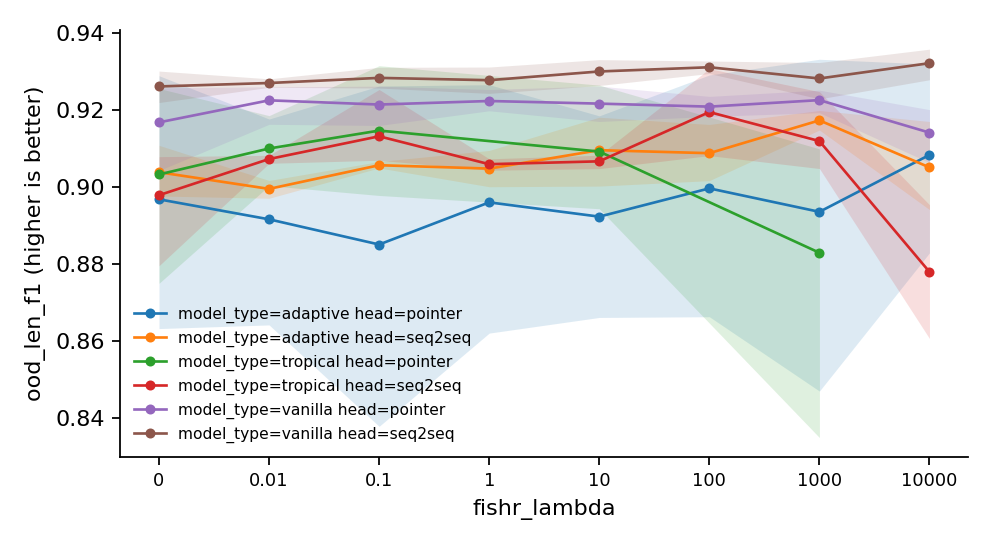
\includegraphics[width=\textwidth]{metric_ood_len_f1.png}
\caption{\texttt{ood\_len\_f1} against \texttt{fishr\_lambda}: the mean over seeds with a 95\% bootstrap CI, one line per combination of the other factors.}
\label{fig:ood_len_f1}
\end{figure}

{\small
\begin{longtable}{lllrlrrr}
\caption{\texttt{ood\_len\_f1} per cell: mean, 95\% bootstrap CI, SD, seeds, diverged runs.}\label{tab:summary-ood_len_f1}\\
\toprule
\texttt{model\_type} & \texttt{head} & \texttt{fishr\_lambda} & mean & 95\% CI & SD & $n$ & div.\\
\midrule
\endhead
adaptive & pointer & 0 & 0.8967 & [0.863, 0.929] & 0.0429 & 5 & 0\\
adaptive & pointer & 0.01 & 0.8915 & [0.864, 0.918] & 0.0359 & 5 & 0\\
adaptive & pointer & 0.1 & 0.885 & [0.838, 0.926] & 0.057 & 5 & 0\\
adaptive & pointer & 1 & 0.896 & [0.862, 0.927] & 0.0417 & 5 & 0\\
adaptive & pointer & 10 & 0.8922 & [0.866, 0.918] & 0.0328 & 5 & 0\\
adaptive & pointer & 100 & 0.8996 & [0.866, 0.929] & 0.0408 & 5 & 0\\
adaptive & pointer & 1000 & 0.8935 & [0.847, 0.933] & 0.0555 & 5 & 0\\
adaptive & pointer & 1e+04 & 0.9083 & [0.883, 0.932] & 0.0317 & 5 & 0\\
adaptive & seq2seq & 0 & 0.9038 & [0.898, 0.911] & 0.00814 & 5 & 0\\
adaptive & seq2seq & 0.01 & 0.8995 & [0.897, 0.902] & 0.00296 & 5 & 0\\
adaptive & seq2seq & 0.1 & 0.9056 & [0.905, 0.907] & 0.00109 & 5 & 0\\
adaptive & seq2seq & 1 & 0.9047 & [0.9, 0.909] & 0.00602 & 5 & 0\\
adaptive & seq2seq & 10 & 0.9095 & [0.9, 0.918] & 0.0116 & 5 & 0\\
adaptive & seq2seq & 100 & 0.9087 & [0.902, 0.916] & 0.00956 & 5 & 0\\
adaptive & seq2seq & 1000 & 0.9173 & [0.915, 0.92] & 0.00334 & 5 & 0\\
adaptive & seq2seq & 1e+04 & 0.905 & [0.894, 0.917] & 0.0155 & 5 & 0\\
tropical & pointer & 0 & 0.9032 & [0.875, 0.926] & 0.0337 & 5 & 0\\
tropical & pointer & 0.01 & 0.9099 & [0.9, 0.918] & 0.011 & 4 & 0\\
tropical & pointer & 0.1 & 0.9146 & [0.898, 0.931] & 0.0202 & 4 & 0\\
tropical & pointer & 10 & 0.9092 & [0.894, 0.926] & 0.02 & 4 & 0\\
tropical & pointer & 1000 & 0.8829 & [0.835, 0.91] & 0.0417 & 3 & 0\\
tropical & seq2seq & 0 & 0.8978 & [0.879, 0.908] & 0.0204 & 5 & 0\\
tropical & seq2seq & 0.01 & 0.9072 & [0.906, 0.908] & 0.00129 & 5 & 0\\
tropical & seq2seq & 0.1 & 0.9131 & [0.907, 0.925] & 0.0136 & 5 & 0\\
tropical & seq2seq & 1 & 0.9059 & [0.904, 0.907] & 0.00199 & 5 & 0\\
tropical & seq2seq & 10 & 0.9066 & [0.905, 0.908] & 0.00219 & 5 & 0\\
tropical & seq2seq & 100 & 0.9194 & [0.908, 0.931] & 0.0153 & 5 & 0\\
tropical & seq2seq & 1000 & 0.9119 & [0.905, 0.925] & 0.0142 & 5 & 0\\
tropical & seq2seq & 1e+04 & 0.8779 & [0.861, 0.895] & 0.0235 & 5 & 0\\
vanilla & pointer & 0 & 0.9167 & [0.904, 0.926] & 0.0137 & 5 & 0\\
vanilla & pointer & 0.01 & 0.9225 & [0.916, 0.926] & 0.00687 & 5 & 0\\
vanilla & pointer & 0.1 & 0.9214 & [0.916, 0.926] & 0.00645 & 5 & 0\\
vanilla & pointer & 1 & 0.9223 & [0.92, 0.925] & 0.0035 & 5 & 0\\
vanilla & pointer & 10 & 0.9216 & [0.917, 0.926] & 0.00646 & 5 & 0\\
vanilla & pointer & 100 & 0.9208 & [0.918, 0.923] & 0.00337 & 5 & 0\\
vanilla & pointer & 1000 & 0.9225 & [0.919, 0.925] & 0.00395 & 5 & 0\\
vanilla & pointer & 1e+04 & 0.9141 & [0.906, 0.92] & 0.00872 & 5 & 0\\
vanilla & seq2seq & 0 & 0.9261 & [0.922, 0.93] & 0.00543 & 5 & 0\\
vanilla & seq2seq & 0.01 & 0.927 & [0.926, 0.928] & 0.00143 & 5 & 0\\
vanilla & seq2seq & 0.1 & 0.9283 & [0.926, 0.931] & 0.00354 & 5 & 0\\
vanilla & seq2seq & 1 & 0.9277 & [0.924, 0.931] & 0.00433 & 5 & 0\\
vanilla & seq2seq & 10 & 0.93 & [0.926, 0.933] & 0.00459 & 5 & 0\\
vanilla & seq2seq & 100 & 0.9311 & [0.929, 0.933] & 0.00209 & 5 & 0\\
vanilla & seq2seq & 1000 & 0.9281 & [0.923, 0.932] & 0.00637 & 5 & 0\\
vanilla & seq2seq & 1e+04 & 0.9321 & [0.928, 0.936] & 0.00505 & 5 & 0\\
\bottomrule
\end{longtable}
}

{\small
\begin{longtable}{lllrrrl}
\caption{\texttt{ood\_len\_f1}: each level of \texttt{fishr\_lambda} against its control (0), within each combination of the other factors. parametric: Dunnett vs control.}\label{tab:control-ood_len_f1}\\
\toprule
\texttt{model\_type} & \texttt{head} & \texttt{fishr\_lambda} & difference & 95\% CI & $p$ & \\
\midrule
\endhead
adaptive & pointer & 0.01 & -0.005196 & [-0.0807, 0.0703] & 1.0000 & \\
adaptive & pointer & 0.1 & -0.01174 & [-0.0872, 0.0637] & 0.9981 & \\
adaptive & pointer & 1 & $-7.894\times10^{-4}$ & [-0.0763, 0.0747] & 1.0000 & \\
adaptive & pointer & 10 & -0.0045 & [-0.08, 0.071] & 1.0000 & \\
adaptive & pointer & 100 & 0.002846 & [-0.0726, 0.0783] & 1.0000 & \\
adaptive & pointer & 1000 & -0.003251 & [-0.0787, 0.0722] & 1.0000 & \\
adaptive & pointer & 1e+04 & 0.01154 & [-0.064, 0.087] & 0.9983 & \\
adaptive & seq2seq & 0.01 & -0.004328 & [-0.0193, 0.0107] & 0.9444 & \\
adaptive & seq2seq & 0.1 & 0.00182 & [-0.0132, 0.0168] & 0.9996 & \\
adaptive & seq2seq & 1 & $9.440\times10^{-4}$ & [-0.0141, 0.016] & 1.0000 & \\
adaptive & seq2seq & 10 & 0.005731 & [-0.00928, 0.0207] & 0.8231 & \\
adaptive & seq2seq & 100 & 0.004947 & [-0.0101, 0.02] & 0.8999 & \\
adaptive & seq2seq & 1000 & 0.01348 & [-0.00154, 0.0285] & 0.0930 & \\
adaptive & seq2seq & 1e+04 & 0.001255 & [-0.0138, 0.0163] & 1.0000 & \\
tropical & pointer & 0.01 & 0.006744 & [-0.0427, 0.0562] & 0.9882 & \\
tropical & pointer & 0.1 & 0.0114 & [-0.0381, 0.0609] & 0.9270 & \\
tropical & pointer & 10 & 0.005948 & [-0.0435, 0.0554] & 0.9926 & \\
tropical & pointer & 1000 & -0.02035 & [-0.0742, 0.0335] & 0.7097 & \\
tropical & seq2seq & 0.01 & 0.009397 & [-0.0153, 0.0341] & 0.8249 & \\
tropical & seq2seq & 0.1 & 0.0153 & [-0.00938, 0.04] & 0.3827 & \\
tropical & seq2seq & 1 & 0.008052 & [-0.0166, 0.0327] & 0.9041 & \\
tropical & seq2seq & 10 & 0.008799 & [-0.0159, 0.0335] & 0.8629 & \\
tropical & seq2seq & 100 & 0.0216 & [-0.00309, 0.0463] & 0.1062 & \\
tropical & seq2seq & 1000 & 0.01406 & [-0.0106, 0.0387] & 0.4690 & \\
tropical & seq2seq & 1e+04 & -0.01993 & [-0.0446, 0.00475] & 0.1544 & \\
vanilla & pointer & 0.01 & 0.005723 & [-0.00712, 0.0186] & 0.7075 & \\
vanilla & pointer & 0.1 & 0.004625 & [-0.00822, 0.0175] & 0.8575 & \\
vanilla & pointer & 1 & 0.005547 & [-0.0073, 0.0184] & 0.7337 & \\
vanilla & pointer & 10 & 0.004868 & [-0.00798, 0.0177] & 0.8276 & \\
vanilla & pointer & 100 & 0.004085 & [-0.00876, 0.0169] & 0.9138 & \\
vanilla & pointer & 1000 & 0.005777 & [-0.00707, 0.0186] & 0.6995 & \\
vanilla & pointer & 1e+04 & -0.002669 & [-0.0155, 0.0102] & 0.9898 & \\
vanilla & seq2seq & 0.01 & $8.942\times10^{-4}$ & [-0.00678, 0.00857] & 0.9997 & \\
vanilla & seq2seq & 0.1 & 0.002226 & [-0.00545, 0.0099] & 0.9430 & \\
vanilla & seq2seq & 1 & 0.001625 & [-0.00605, 0.0093] & 0.9886 & \\
vanilla & seq2seq & 10 & 0.003893 & [-0.00378, 0.0116] & 0.5871 & \\
vanilla & seq2seq & 100 & 0.004989 & [-0.00269, 0.0127] & 0.3359 & \\
vanilla & seq2seq & 1000 & 0.002072 & [-0.0056, 0.00975] & 0.9594 & \\
vanilla & seq2seq & 1e+04 & 0.006049 & [-0.00163, 0.0137] & 0.1711 & \\
\bottomrule
\end{longtable}
}

{\small
\begin{longtable}{llrrrrr}
\caption{\texttt{ood\_len\_f1} against log10 \texttt{fishr\_lambda}: parametric: OLS slope t-test, seed-bootstrap CI, with the Jonckheere--Terpstra ordered-trend $\tau$ and $p$.}\label{tab:trend-ood_len_f1}\\
\toprule
\texttt{model\_type} & \texttt{head} & estimate & 95\% CI & $p$ & JT $\tau$ & JT $p$\\
\midrule
\endhead
adaptive & pointer & 0.002529 & [0.0011, 0.00408] & 0.4610 & 0.227 & 0.0928\\
adaptive & seq2seq & 0.001574 & [$7.00\times10^{-4}$, 0.00275] & 0.0461 & 0.318 & 0.0190\\
tropical & pointer & -0.005129 & [-0.0111, $9.70\times10^{-4}$] & 0.1365 & -0.214 & 0.3931\\
tropical & seq2seq & -0.002747 & [-0.00491, $-4.73\times10^{-4}$] & 0.0569 & -0.25 & 0.0584\\
vanilla & pointer & $-8.691\times10^{-4}$ & [-0.00246, $5.01\times10^{-4}$] & 0.0906 & -0.253 & 0.0588\\
vanilla & seq2seq & $6.615\times10^{-4}$ & [$-5.71\times10^{-6}$, 0.00139] & 0.0633 & 0.322 & 0.0120\\
\bottomrule
\end{longtable}
}

{\small
\begin{longtable}{lrrrl}
\caption{\texttt{ood\_len\_f1}: paired contrasts by seed, Holm-corrected across the cells. parametric: paired t-test by seed, Holm.}\label{tab:paired-ood_len_f1}\\
\toprule
contrast (within) & difference & 95\% CI & $p$ & \\
\midrule
\endhead
\stackcell{model\_type: tropical - vanilla\\\footnotesize head=pointer fishr\_lambda=0 } & -0.01354 & [-0.055, 0.0279] & 1.0000 & \\
\stackcell{model\_type: tropical - vanilla\\\footnotesize head=pointer fishr\_lambda=0.01 } & -0.01557 & [-0.033, 0.00183] & 0.4563 & \\
\stackcell{model\_type: tropical - vanilla\\\footnotesize head=pointer fishr\_lambda=0.1 } & -0.007895 & [-0.047, 0.0312] & 1.0000 & \\
\stackcell{model\_type: tropical - vanilla\\\footnotesize head=pointer fishr\_lambda=10 } & -0.01327 & [-0.0503, 0.0237] & 1.0000 & \\
\stackcell{model\_type: tropical - vanilla\\\footnotesize head=pointer fishr\_lambda=1000 } & -0.0406 & [-0.147, 0.0657] & 0.9681 & \\
\stackcell{model\_type: tropical - vanilla\\\footnotesize head=seq2seq fishr\_lambda=0 } & -0.02826 & [-0.0553, -0.00119] & 0.3564 & \\
\stackcell{model\_type: tropical - vanilla\\\footnotesize head=seq2seq fishr\_lambda=0.01 } & -0.01975 & [-0.0223, -0.0172] & 0.0003 & *\\
\stackcell{model\_type: tropical - vanilla\\\footnotesize head=seq2seq fishr\_lambda=0.1 } & -0.01518 & [-0.0292, -0.00117] & 0.3564 & \\
\stackcell{model\_type: tropical - vanilla\\\footnotesize head=seq2seq fishr\_lambda=1 } & -0.02183 & [-0.0275, -0.0162] & 0.0051 & *\\
\stackcell{model\_type: tropical - vanilla\\\footnotesize head=seq2seq fishr\_lambda=10 } & -0.02335 & [-0.0294, -0.0173] & 0.0051 & *\\
\stackcell{model\_type: tropical - vanilla\\\footnotesize head=seq2seq fishr\_lambda=100 } & -0.01165 & [-0.032, 0.00866] & 0.9326 & \\
\stackcell{model\_type: tropical - vanilla\\\footnotesize head=seq2seq fishr\_lambda=1000 } & -0.01627 & [-0.0352, 0.0027] & 0.4563 & \\
\stackcell{model\_type: tropical - vanilla\\\footnotesize head=seq2seq fishr\_lambda=1e+04 } & -0.05424 & [-0.0803, -0.0282] & 0.0445 & *\\
\stackcell{model\_type: adaptive - vanilla\\\footnotesize head=pointer fishr\_lambda=0 } & -0.02 & [-0.0778, 0.0378] & 1.0000 & \\
\stackcell{model\_type: adaptive - vanilla\\\footnotesize head=pointer fishr\_lambda=0.01 } & -0.03092 & [-0.0696, 0.00776] & 0.7252 & \\
\stackcell{model\_type: adaptive - vanilla\\\footnotesize head=pointer fishr\_lambda=0.1 } & -0.03637 & [-0.107, 0.0343] & 1.0000 & \\
\stackcell{model\_type: adaptive - vanilla\\\footnotesize head=pointer fishr\_lambda=1 } & -0.02634 & [-0.0765, 0.0239] & 1.0000 & \\
\stackcell{model\_type: adaptive - vanilla\\\footnotesize head=pointer fishr\_lambda=10 } & -0.02937 & [-0.0709, 0.0122] & 0.8473 & \\
\stackcell{model\_type: adaptive - vanilla\\\footnotesize head=pointer fishr\_lambda=100 } & -0.02124 & [-0.0696, 0.0272] & 1.0000 & \\
\stackcell{model\_type: adaptive - vanilla\\\footnotesize head=pointer fishr\_lambda=1000 } & -0.02903 & [-0.0986, 0.0405] & 1.0000 & \\
\stackcell{model\_type: adaptive - vanilla\\\footnotesize head=pointer fishr\_lambda=1e+04 } & -0.005795 & [-0.0471, 0.0355] & 1.0000 & \\
\stackcell{model\_type: adaptive - vanilla\\\footnotesize head=seq2seq fishr\_lambda=0 } & -0.02229 & [-0.0365, -0.00803] & 0.1471 & \\
\stackcell{model\_type: adaptive - vanilla\\\footnotesize head=seq2seq fishr\_lambda=0.01 } & -0.02751 & [-0.0316, -0.0235] & 0.0007 & *\\
\stackcell{model\_type: adaptive - vanilla\\\footnotesize head=seq2seq fishr\_lambda=0.1 } & -0.02269 & [-0.0263, -0.0191] & 0.0009 & *\\
\stackcell{model\_type: adaptive - vanilla\\\footnotesize head=seq2seq fishr\_lambda=1 } & -0.02297 & [-0.0283, -0.0176] & 0.0039 & *\\
\stackcell{model\_type: adaptive - vanilla\\\footnotesize head=seq2seq fishr\_lambda=10 } & -0.02045 & [-0.0389, -0.00198] & 0.3341 & \\
\stackcell{model\_type: adaptive - vanilla\\\footnotesize head=seq2seq fishr\_lambda=100 } & -0.02233 & [-0.035, -0.00968] & 0.1044 & \\
\stackcell{model\_type: adaptive - vanilla\\\footnotesize head=seq2seq fishr\_lambda=1000 } & -0.01088 & [-0.0198, -0.00197] & 0.2751 & \\
\stackcell{model\_type: adaptive - vanilla\\\footnotesize head=seq2seq fishr\_lambda=1e+04 } & -0.02708 & [-0.0464, -0.00773] & 0.1954 & \\
\stackcell{head: pointer - seq2seq\\\footnotesize model\_type=adaptive fishr\_lambda=0 } & -0.007042 & [-0.0552, 0.0411] & 1.0000 & \\
\stackcell{head: pointer - seq2seq\\\footnotesize model\_type=adaptive fishr\_lambda=0.01 } & -0.00791 & [-0.0497, 0.0339] & 1.0000 & \\
\stackcell{head: pointer - seq2seq\\\footnotesize model\_type=adaptive fishr\_lambda=0.1 } & -0.0206 & [-0.0912, 0.05] & 1.0000 & \\
\stackcell{head: pointer - seq2seq\\\footnotesize model\_type=adaptive fishr\_lambda=1 } & -0.008775 & [-0.0632, 0.0457] & 1.0000 & \\
\stackcell{head: pointer - seq2seq\\\footnotesize model\_type=adaptive fishr\_lambda=10 } & -0.01727 & [-0.0714, 0.0368] & 1.0000 & \\
\stackcell{head: pointer - seq2seq\\\footnotesize model\_type=adaptive fishr\_lambda=100 } & -0.009143 & [-0.058, 0.0397] & 1.0000 & \\
\stackcell{head: pointer - seq2seq\\\footnotesize model\_type=adaptive fishr\_lambda=1000 } & -0.02377 & [-0.0926, 0.045] & 1.0000 & \\
\stackcell{head: pointer - seq2seq\\\footnotesize model\_type=adaptive fishr\_lambda=1e+04 } & 0.003241 & [-0.0333, 0.0398] & 1.0000 & \\
\stackcell{head: pointer - seq2seq\\\footnotesize model\_type=tropical fishr\_lambda=0 } & 0.005388 & [-0.0509, 0.0617] & 1.0000 & \\
\stackcell{head: pointer - seq2seq\\\footnotesize model\_type=tropical fishr\_lambda=0.01 } & 0.003037 & [-0.0156, 0.0217] & 1.0000 & \\
\stackcell{head: pointer - seq2seq\\\footnotesize model\_type=tropical fishr\_lambda=0.1 } & $2.653\times10^{-5}$ & [-0.0208, 0.0209] & 1.0000 & \\
\stackcell{head: pointer - seq2seq\\\footnotesize model\_type=tropical fishr\_lambda=10 } & 0.00275 & [-0.0326, 0.0381] & 1.0000 & \\
\stackcell{head: pointer - seq2seq\\\footnotesize model\_type=tropical fishr\_lambda=1000 } & -0.02215 & [-0.129, 0.0843] & 1.0000 & \\
\stackcell{head: pointer - seq2seq\\\footnotesize model\_type=vanilla fishr\_lambda=0 } & -0.00933 & [-0.0318, 0.0131] & 1.0000 & \\
\stackcell{head: pointer - seq2seq\\\footnotesize model\_type=vanilla fishr\_lambda=0.01 } & -0.004501 & [-0.0142, 0.00521] & 1.0000 & \\
\stackcell{head: pointer - seq2seq\\\footnotesize model\_type=vanilla fishr\_lambda=0.1 } & -0.00693 & [-0.0182, 0.00433] & 1.0000 & \\
\stackcell{head: pointer - seq2seq\\\footnotesize model\_type=vanilla fishr\_lambda=1 } & -0.005407 & [-0.0118, $9.74\times10^{-4}$] & 1.0000 & \\
\stackcell{head: pointer - seq2seq\\\footnotesize model\_type=vanilla fishr\_lambda=10 } & -0.008354 & [-0.0206, 0.00389] & 1.0000 & \\
\stackcell{head: pointer - seq2seq\\\footnotesize model\_type=vanilla fishr\_lambda=100 } & -0.01023 & [-0.0148, -0.00563] & 0.0736 & \\
\stackcell{head: pointer - seq2seq\\\footnotesize model\_type=vanilla fishr\_lambda=1000 } & -0.005624 & [-0.0164, 0.00519] & 1.0000 & \\
\stackcell{head: pointer - seq2seq\\\footnotesize model\_type=vanilla fishr\_lambda=1e+04 } & -0.01805 & [-0.0323, -0.00379] & 0.4920 & \\
\bottomrule
\end{longtable}
}

\clearpage
\appendix
\section{Other metrics}
\subsection{\texttt{ood\_len\_exact}}
\begin{figure}[tbp]
\centering
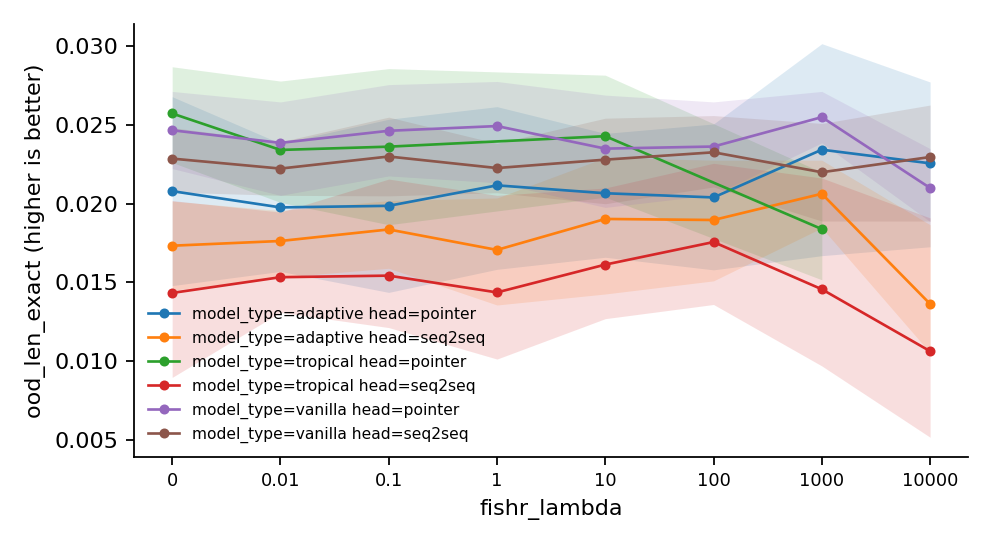
\includegraphics[width=\textwidth]{metric_ood_len_exact.png}
\caption{\texttt{ood\_len\_exact} against \texttt{fishr\_lambda}: the mean over seeds with a 95\% bootstrap CI, one line per combination of the other factors.}
\label{fig:ood_len_exact}
\end{figure}

{\small
\begin{longtable}{lllrlrrr}
\caption{\texttt{ood\_len\_exact} per cell: mean, 95\% bootstrap CI, SD, seeds, diverged runs.}\label{tab:summary-ood_len_exact}\\
\toprule
\texttt{model\_type} & \texttt{head} & \texttt{fishr\_lambda} & mean & 95\% CI & SD & $n$ & div.\\
\midrule
\endhead
adaptive & pointer & 0 & 0.0208 & [0.0148, 0.0268] & 0.00784 & 5 & 0\\
adaptive & pointer & 0.01 & 0.01977 & [0.0157, 0.0238] & 0.00542 & 5 & 0\\
adaptive & pointer & 0.1 & 0.01987 & [0.0144, 0.0254] & 0.00711 & 5 & 0\\
adaptive & pointer & 1 & 0.02117 & [0.0158, 0.0262] & 0.00679 & 5 & 0\\
adaptive & pointer & 10 & 0.02067 & [0.0166, 0.0245] & 0.0052 & 5 & 0\\
adaptive & pointer & 100 & 0.0204 & [0.0158, 0.0251] & 0.00602 & 5 & 0\\
adaptive & pointer & 1000 & 0.02343 & [0.0167, 0.0302] & 0.00901 & 5 & 0\\
adaptive & pointer & 1e+04 & 0.02257 & [0.0173, 0.0277] & 0.00693 & 5 & 0\\
adaptive & seq2seq & 0 & 0.01733 & [0.0145, 0.0202] & 0.00385 & 5 & 0\\
adaptive & seq2seq & 0.01 & 0.01763 & [0.0153, 0.0196] & 0.00279 & 5 & 0\\
adaptive & seq2seq & 0.1 & 0.01837 & [0.0159, 0.0202] & 0.00289 & 5 & 0\\
adaptive & seq2seq & 1 & 0.01707 & [0.0136, 0.0204] & 0.00459 & 5 & 0\\
adaptive & seq2seq & 10 & 0.01903 & [0.0143, 0.0229] & 0.00576 & 5 & 0\\
adaptive & seq2seq & 100 & 0.01897 & [0.0151, 0.0228] & 0.00497 & 5 & 0\\
adaptive & seq2seq & 1000 & 0.02063 & [0.0185, 0.0228] & 0.00286 & 5 & 0\\
adaptive & seq2seq & 1e+04 & 0.01363 & [0.0105, 0.0187] & 0.00568 & 5 & 0\\
tropical & pointer & 0 & 0.02573 & [0.0226, 0.0287] & 0.00414 & 5 & 0\\
tropical & pointer & 0.01 & 0.02342 & [0.0201, 0.0278] & 0.00484 & 4 & 0\\
tropical & pointer & 0.1 & 0.02363 & [0.0187, 0.0286] & 0.0059 & 4 & 0\\
tropical & pointer & 10 & 0.02429 & [0.0204, 0.0282] & 0.00459 & 4 & 0\\
tropical & pointer & 1000 & 0.01839 & [0.0152, 0.022] & 0.00343 & 3 & 0\\
tropical & seq2seq & 0 & 0.01433 & [0.00897, 0.0202] & 0.00669 & 5 & 0\\
tropical & seq2seq & 0.01 & 0.01533 & [0.0131, 0.0195] & 0.00458 & 5 & 0\\
tropical & seq2seq & 0.1 & 0.01543 & [0.0121, 0.0216] & 0.00685 & 5 & 0\\
tropical & seq2seq & 1 & 0.01437 & [0.0101, 0.0205] & 0.00681 & 5 & 0\\
tropical & seq2seq & 10 & 0.01613 & [0.0127, 0.021] & 0.00535 & 5 & 0\\
tropical & seq2seq & 100 & 0.01757 & [0.0136, 0.0226] & 0.00579 & 5 & 0\\
tropical & seq2seq & 1000 & 0.01457 & [0.0097, 0.0216] & 0.00798 & 5 & 0\\
tropical & seq2seq & 1e+04 & 0.01063 & [0.00517, 0.0191] & 0.0094 & 5 & 0\\
vanilla & pointer & 0 & 0.02467 & [0.0222, 0.0271] & 0.00313 & 5 & 0\\
vanilla & pointer & 0.01 & 0.02387 & [0.0205, 0.0265] & 0.00392 & 5 & 0\\
vanilla & pointer & 0.1 & 0.02463 & [0.0218, 0.0276] & 0.00354 & 5 & 0\\
vanilla & pointer & 1 & 0.02493 & [0.0213, 0.0278] & 0.00406 & 5 & 0\\
vanilla & pointer & 10 & 0.0235 & [0.0198, 0.0269] & 0.00461 & 5 & 0\\
vanilla & pointer & 100 & 0.02363 & [0.0206, 0.0265] & 0.0039 & 5 & 0\\
vanilla & pointer & 1000 & 0.0255 & [0.0239, 0.0271] & 0.0021 & 5 & 0\\
vanilla & pointer & 1e+04 & 0.021 & [0.0189, 0.0235] & 0.003 & 5 & 0\\
vanilla & seq2seq & 0 & 0.02287 & [0.0207, 0.0248] & 0.00272 & 5 & 0\\
vanilla & seq2seq & 0.01 & 0.02223 & [0.0205, 0.0239] & 0.00221 & 5 & 0\\
vanilla & seq2seq & 0.1 & 0.023 & [0.0205, 0.0255] & 0.00328 & 5 & 0\\
vanilla & seq2seq & 1 & 0.02227 & [0.0207, 0.0238] & 0.00207 & 5 & 0\\
vanilla & seq2seq & 10 & 0.0228 & [0.02, 0.0254] & 0.0037 & 5 & 0\\
vanilla & seq2seq & 100 & 0.02327 & [0.0211, 0.0256] & 0.00293 & 5 & 0\\
vanilla & seq2seq & 1000 & 0.022 & [0.0189, 0.0251] & 0.00426 & 5 & 0\\
vanilla & seq2seq & 1e+04 & 0.02297 & [0.0189, 0.0263] & 0.00456 & 5 & 0\\
\bottomrule
\end{longtable}
}

{\small
\begin{longtable}{lllrrrl}
\caption{\texttt{ood\_len\_exact}: each level of \texttt{fishr\_lambda} against its control (0), within each combination of the other factors. parametric: Dunnett vs control.}\label{tab:control-ood_len_exact}\\
\toprule
\texttt{model\_type} & \texttt{head} & \texttt{fishr\_lambda} & difference & 95\% CI & $p$ & \\
\midrule
\endhead
adaptive & pointer & 0.01 & -0.001033 & [-0.0131, 0.011] & 1.0000 & \\
adaptive & pointer & 0.1 & $-9.333\times10^{-4}$ & [-0.013, 0.0111] & 1.0000 & \\
adaptive & pointer & 1 & $3.667\times10^{-4}$ & [-0.0117, 0.0124] & 1.0000 & \\
adaptive & pointer & 10 & $-1.333\times10^{-4}$ & [-0.0122, 0.0119] & 1.0000 & \\
adaptive & pointer & 100 & $-4.000\times10^{-4}$ & [-0.0124, 0.0116] & 1.0000 & \\
adaptive & pointer & 1000 & 0.002633 & [-0.00941, 0.0147] & 0.9864 & \\
adaptive & pointer & 1e+04 & 0.001767 & [-0.0103, 0.0138] & 0.9987 & \\
adaptive & seq2seq & 0.01 & $3.000\times10^{-4}$ & [-0.00727, 0.00787] & 1.0000 & \\
adaptive & seq2seq & 0.1 & 0.001033 & [-0.00654, 0.00861] & 0.9992 & \\
adaptive & seq2seq & 1 & $-2.667\times10^{-4}$ & [-0.00784, 0.00731] & 1.0000 & \\
adaptive & seq2seq & 10 & 0.0017 & [-0.00587, 0.00927] & 0.9843 & \\
adaptive & seq2seq & 100 & 0.001633 & [-0.00594, 0.00921] & 0.9874 & \\
adaptive & seq2seq & 1000 & 0.0033 & [-0.00427, 0.0109] & 0.7263 & \\
adaptive & seq2seq & 1e+04 & -0.0037 & [-0.0113, 0.00387] & 0.6236 & \\
tropical & pointer & 0.01 & -0.002317 & [-0.011, 0.00633] & 0.8840 & \\
tropical & pointer & 0.1 & -0.002108 & [-0.0108, 0.00654] & 0.9130 & \\
tropical & pointer & 10 & -0.001442 & [-0.0101, 0.00721] & 0.9757 & \\
tropical & pointer & 1000 & -0.007344 & [-0.0168, 0.00207] & 0.1521 & \\
tropical & seq2seq & 0.01 & 0.001 & [-0.0109, 0.0129] & 1.0000 & \\
tropical & seq2seq & 0.1 & 0.0011 & [-0.0108, 0.013] & 0.9999 & \\
tropical & seq2seq & 1 & $3.333\times10^{-5}$ & [-0.0119, 0.012] & 1.0000 & \\
tropical & seq2seq & 10 & 0.0018 & [-0.0101, 0.0137] & 0.9985 & \\
tropical & seq2seq & 100 & 0.003233 & [-0.0087, 0.0152] & 0.9586 & \\
tropical & seq2seq & 1000 & $2.333\times10^{-4}$ & [-0.0117, 0.0122] & 1.0000 & \\
tropical & seq2seq & 1e+04 & -0.0037 & [-0.0156, 0.00823] & 0.9228 & \\
vanilla & pointer & 0.01 & $-8.000\times10^{-4}$ & [-0.0071, 0.0055] & 0.9995 & \\
vanilla & pointer & 0.1 & $-3.333\times10^{-5}$ & [-0.00633, 0.00627] & 1.0000 & \\
vanilla & pointer & 1 & $2.667\times10^{-4}$ & [-0.00603, 0.00657] & 1.0000 & \\
vanilla & pointer & 10 & -0.001167 & [-0.00747, 0.00513] & 0.9947 & \\
vanilla & pointer & 100 & -0.001033 & [-0.00733, 0.00527] & 0.9974 & \\
vanilla & pointer & 1000 & $8.333\times10^{-4}$ & [-0.00547, 0.00713] & 0.9993 & \\
vanilla & pointer & 1e+04 & -0.003667 & [-0.00997, 0.00263] & 0.4468 & \\
vanilla & seq2seq & 0.01 & $-6.333\times10^{-4}$ & [-0.00645, 0.00518] & 0.9998 & \\
vanilla & seq2seq & 0.1 & $1.333\times10^{-4}$ & [-0.00568, 0.00595] & 1.0000 & \\
vanilla & seq2seq & 1 & $-6.000\times10^{-4}$ & [-0.00641, 0.00521] & 0.9999 & \\
vanilla & seq2seq & 10 & $-6.667\times10^{-5}$ & [-0.00588, 0.00575] & 1.0000 & \\
vanilla & seq2seq & 100 & $4.000\times10^{-4}$ & [-0.00541, 0.00621] & 1.0000 & \\
vanilla & seq2seq & 1000 & $-8.667\times10^{-4}$ & [-0.00668, 0.00495] & 0.9986 & \\
vanilla & seq2seq & 1e+04 & $1.000\times10^{-4}$ & [-0.00571, 0.00591] & 1.0000 & \\
\bottomrule
\end{longtable}
}

{\small
\begin{longtable}{llrrrrr}
\caption{\texttt{ood\_len\_exact} against log10 \texttt{fishr\_lambda}: parametric: OLS slope t-test, seed-bootstrap CI, with the Jonckheere--Terpstra ordered-trend $\tau$ and $p$.}\label{tab:trend-ood_len_exact}\\
\toprule
\texttt{model\_type} & \texttt{head} & estimate & 95\% CI & $p$ & JT $\tau$ & JT $p$\\
\midrule
\endhead
adaptive & pointer & $5.274\times10^{-4}$ & [$1.92\times10^{-4}$, 0.00106] & 0.3260 & 0.105 & 0.4309\\
adaptive & seq2seq & $-1.988\times10^{-4}$ & [$-6.99\times10^{-4}$, $3.52\times10^{-4}$] & 0.6083 & -0.00952 & 0.9558\\
tropical & pointer & $-8.220\times10^{-4}$ & [-0.00155, $5.74\times10^{-4}$] & 0.2424 & -0.274 & 0.2657\\
tropical & seq2seq & $-4.512\times10^{-4}$ & [$-8.65\times10^{-4}$, $1.18\times10^{-5}$] & 0.4221 & -0.156 & 0.2412\\
vanilla & pointer & $-2.917\times10^{-4}$ & [$-6.83\times10^{-4}$, $1.40\times10^{-4}$] & 0.3454 & -0.143 & 0.2879\\
vanilla & seq2seq & $4.286\times10^{-5}$ & [$-4.56\times10^{-4}$, $6.42\times10^{-4}$] & 0.8738 & 0.0533 & 0.6961\\
\bottomrule
\end{longtable}
}

{\small
\begin{longtable}{lrrrl}
\caption{\texttt{ood\_len\_exact}: paired contrasts by seed, Holm-corrected across the cells. parametric: paired t-test by seed, Holm.}\label{tab:paired-ood_len_exact}\\
\toprule
contrast (within) & difference & 95\% CI & $p$ & \\
\midrule
\endhead
\stackcell{model\_type: tropical - vanilla\\\footnotesize head=pointer fishr\_lambda=0 } & 0.001067 & [-0.00417, 0.0063] & 1.0000 & \\
\stackcell{model\_type: tropical - vanilla\\\footnotesize head=pointer fishr\_lambda=0.01 } & -0.002042 & [-0.0106, 0.00649] & 1.0000 & \\
\stackcell{model\_type: tropical - vanilla\\\footnotesize head=pointer fishr\_lambda=0.1 } & -0.002292 & [-0.0125, 0.00791] & 1.0000 & \\
\stackcell{model\_type: tropical - vanilla\\\footnotesize head=pointer fishr\_lambda=10 } & $-8.674\times10^{-19}$ & [-0.00912, 0.00912] & 1.0000 & \\
\stackcell{model\_type: tropical - vanilla\\\footnotesize head=pointer fishr\_lambda=1000 } & -0.007111 & [-0.021, 0.0068] & 0.9306 & \\
\stackcell{model\_type: tropical - vanilla\\\footnotesize head=seq2seq fishr\_lambda=0 } & -0.008533 & [-0.0188, 0.00169] & 0.7331 & \\
\stackcell{model\_type: tropical - vanilla\\\footnotesize head=seq2seq fishr\_lambda=0.01 } & -0.0069 & [-0.0111, -0.00275] & 0.1292 & \\
\stackcell{model\_type: tropical - vanilla\\\footnotesize head=seq2seq fishr\_lambda=0.1 } & -0.007567 & [-0.0146, $-5.33\times10^{-4}$] & 0.4452 & \\
\stackcell{model\_type: tropical - vanilla\\\footnotesize head=seq2seq fishr\_lambda=1 } & -0.0079 & [-0.0155, $-2.93\times10^{-4}$] & 0.4486 & \\
\stackcell{model\_type: tropical - vanilla\\\footnotesize head=seq2seq fishr\_lambda=10 } & -0.006667 & [-0.0152, 0.00188] & 0.7706 & \\
\stackcell{model\_type: tropical - vanilla\\\footnotesize head=seq2seq fishr\_lambda=100 } & -0.0057 & [-0.0146, 0.0032] & 0.9306 & \\
\stackcell{model\_type: tropical - vanilla\\\footnotesize head=seq2seq fishr\_lambda=1000 } & -0.007433 & [-0.0184, 0.00353] & 0.9306 & \\
\stackcell{model\_type: tropical - vanilla\\\footnotesize head=seq2seq fishr\_lambda=1e+04 } & -0.01233 & [-0.0219, -0.00272] & 0.2822 & \\
\stackcell{model\_type: adaptive - vanilla\\\footnotesize head=pointer fishr\_lambda=0 } & -0.003867 & [-0.0104, 0.00264] & 1.0000 & \\
\stackcell{model\_type: adaptive - vanilla\\\footnotesize head=pointer fishr\_lambda=0.01 } & -0.0041 & [-0.0111, 0.00287] & 1.0000 & \\
\stackcell{model\_type: adaptive - vanilla\\\footnotesize head=pointer fishr\_lambda=0.1 } & -0.004767 & [-0.0148, 0.00524] & 1.0000 & \\
\stackcell{model\_type: adaptive - vanilla\\\footnotesize head=pointer fishr\_lambda=1 } & -0.003767 & [-0.0123, 0.00479] & 1.0000 & \\
\stackcell{model\_type: adaptive - vanilla\\\footnotesize head=pointer fishr\_lambda=10 } & -0.002833 & [-0.00991, 0.00424] & 1.0000 & \\
\stackcell{model\_type: adaptive - vanilla\\\footnotesize head=pointer fishr\_lambda=100 } & -0.003233 & [-0.00924, 0.00278] & 1.0000 & \\
\stackcell{model\_type: adaptive - vanilla\\\footnotesize head=pointer fishr\_lambda=1000 } & -0.002067 & [-0.0125, 0.00839] & 1.0000 & \\
\stackcell{model\_type: adaptive - vanilla\\\footnotesize head=pointer fishr\_lambda=1e+04 } & 0.001567 & [-0.00627, 0.0094] & 1.0000 & \\
\stackcell{model\_type: adaptive - vanilla\\\footnotesize head=seq2seq fishr\_lambda=0 } & -0.005533 & [-0.0133, 0.00226] & 1.0000 & \\
\stackcell{model\_type: adaptive - vanilla\\\footnotesize head=seq2seq fishr\_lambda=0.01 } & -0.0046 & [-0.00708, -0.00212] & 0.1082 & \\
\stackcell{model\_type: adaptive - vanilla\\\footnotesize head=seq2seq fishr\_lambda=0.1 } & -0.004633 & [-0.00998, $7.10\times10^{-4}$] & 0.9588 & \\
\stackcell{model\_type: adaptive - vanilla\\\footnotesize head=seq2seq fishr\_lambda=1 } & -0.0052 & [-0.00955, $-8.53\times10^{-4}$] & 0.4401 & \\
\stackcell{model\_type: adaptive - vanilla\\\footnotesize head=seq2seq fishr\_lambda=10 } & -0.003767 & [-0.0135, 0.00594] & 1.0000 & \\
\stackcell{model\_type: adaptive - vanilla\\\footnotesize head=seq2seq fishr\_lambda=100 } & -0.0043 & [-0.0123, 0.00369] & 1.0000 & \\
\stackcell{model\_type: adaptive - vanilla\\\footnotesize head=seq2seq fishr\_lambda=1000 } & -0.001367 & [-0.00871, 0.00597] & 1.0000 & \\
\stackcell{model\_type: adaptive - vanilla\\\footnotesize head=seq2seq fishr\_lambda=1e+04 } & -0.009333 & [-0.0174, -0.00124] & 0.4603 & \\
\stackcell{head: pointer - seq2seq\\\footnotesize model\_type=adaptive fishr\_lambda=0 } & 0.003467 & [-0.00742, 0.0143] & 1.0000 & \\
\stackcell{head: pointer - seq2seq\\\footnotesize model\_type=adaptive fishr\_lambda=0.01 } & 0.002133 & [-0.00587, 0.0101] & 1.0000 & \\
\stackcell{head: pointer - seq2seq\\\footnotesize model\_type=adaptive fishr\_lambda=0.1 } & 0.0015 & [-0.00882, 0.0118] & 1.0000 & \\
\stackcell{head: pointer - seq2seq\\\footnotesize model\_type=adaptive fishr\_lambda=1 } & 0.0041 & [-0.00647, 0.0147] & 1.0000 & \\
\stackcell{head: pointer - seq2seq\\\footnotesize model\_type=adaptive fishr\_lambda=10 } & 0.001633 & [-0.00998, 0.0132] & 1.0000 & \\
\stackcell{head: pointer - seq2seq\\\footnotesize model\_type=adaptive fishr\_lambda=100 } & 0.001433 & [-0.00778, 0.0106] & 1.0000 & \\
\stackcell{head: pointer - seq2seq\\\footnotesize model\_type=adaptive fishr\_lambda=1000 } & 0.0028 & [-0.00819, 0.0138] & 1.0000 & \\
\stackcell{head: pointer - seq2seq\\\footnotesize model\_type=adaptive fishr\_lambda=1e+04 } & 0.008933 & [-0.00219, 0.0201] & 1.0000 & \\
\stackcell{head: pointer - seq2seq\\\footnotesize model\_type=tropical fishr\_lambda=0 } & 0.0114 & [$7.79\times10^{-4}$, 0.022] & 0.8556 & \\
\stackcell{head: pointer - seq2seq\\\footnotesize model\_type=tropical fishr\_lambda=0.01 } & 0.007458 & [-0.00617, 0.0211] & 1.0000 & \\
\stackcell{head: pointer - seq2seq\\\footnotesize model\_type=tropical fishr\_lambda=0.1 } & 0.007542 & [-0.00458, 0.0197] & 1.0000 & \\
\stackcell{head: pointer - seq2seq\\\footnotesize model\_type=tropical fishr\_lambda=10 } & 0.007875 & [$-9.69\times10^{-5}$, 0.0158] & 1.0000 & \\
\stackcell{head: pointer - seq2seq\\\footnotesize model\_type=tropical fishr\_lambda=1000 } & 0.008444 & [-0.0033, 0.0202] & 1.0000 & \\
\stackcell{head: pointer - seq2seq\\\footnotesize model\_type=vanilla fishr\_lambda=0 } & 0.0018 & [-0.00398, 0.00758] & 1.0000 & \\
\stackcell{head: pointer - seq2seq\\\footnotesize model\_type=vanilla fishr\_lambda=0.01 } & 0.001633 & [-0.00401, 0.00728] & 1.0000 & \\
\stackcell{head: pointer - seq2seq\\\footnotesize model\_type=vanilla fishr\_lambda=0.1 } & 0.001633 & [-0.00428, 0.00755] & 1.0000 & \\
\stackcell{head: pointer - seq2seq\\\footnotesize model\_type=vanilla fishr\_lambda=1 } & 0.002667 & [-0.00238, 0.00771] & 1.0000 & \\
\stackcell{head: pointer - seq2seq\\\footnotesize model\_type=vanilla fishr\_lambda=10 } & $7.000\times10^{-4}$ & [-0.0076, 0.009] & 1.0000 & \\
\stackcell{head: pointer - seq2seq\\\footnotesize model\_type=vanilla fishr\_lambda=100 } & $3.667\times10^{-4}$ & [-0.00471, 0.00545] & 1.0000 & \\
\stackcell{head: pointer - seq2seq\\\footnotesize model\_type=vanilla fishr\_lambda=1000 } & 0.0035 & [-0.00324, 0.0102] & 1.0000 & \\
\stackcell{head: pointer - seq2seq\\\footnotesize model\_type=vanilla fishr\_lambda=1e+04 } & -0.001967 & [-0.00787, 0.00394] & 1.0000 & \\
\bottomrule
\end{longtable}
}

\subsection{\texttt{ood\_val\_f1}}
\begin{figure}[tbp]
\centering
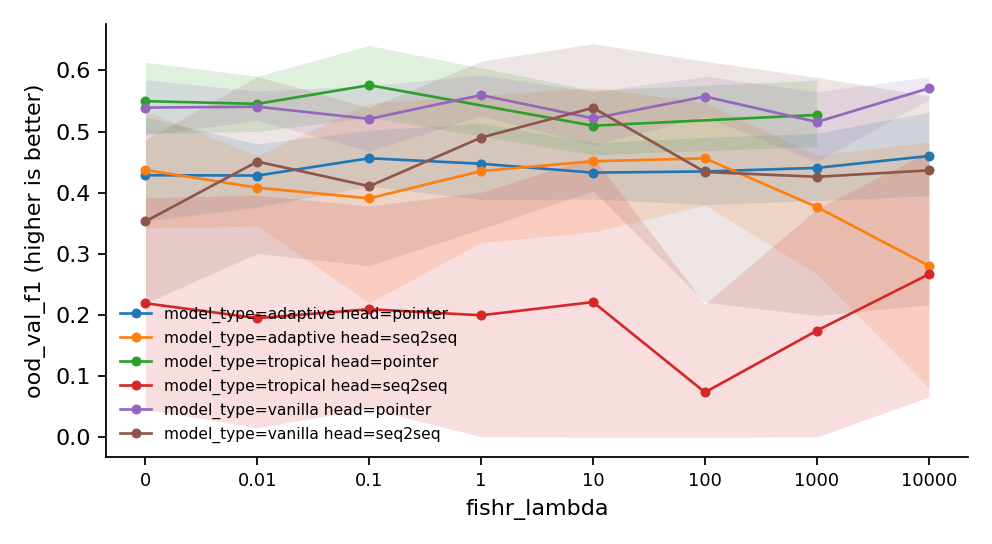
\includegraphics[width=\textwidth]{metric_ood_val_f1.png}
\caption{\texttt{ood\_val\_f1} against \texttt{fishr\_lambda}: the mean over seeds with a 95\% bootstrap CI, one line per combination of the other factors.}
\label{fig:ood_val_f1}
\end{figure}

{\small
\begin{longtable}{lllrlrrr}
\caption{\texttt{ood\_val\_f1} per cell: mean, 95\% bootstrap CI, SD, seeds, diverged runs.}\label{tab:summary-ood_val_f1}\\
\toprule
\texttt{model\_type} & \texttt{head} & \texttt{fishr\_lambda} & mean & 95\% CI & SD & $n$ & div.\\
\midrule
\endhead
adaptive & pointer & 0 & 0.4286 & [0.353, 0.524] & 0.113 & 5 & 0\\
adaptive & pointer & 0.01 & 0.428 & [0.376, 0.48] & 0.0685 & 5 & 0\\
adaptive & pointer & 0.1 & 0.4563 & [0.41, 0.502] & 0.062 & 5 & 0\\
adaptive & pointer & 1 & 0.4473 & [0.389, 0.514] & 0.0799 & 5 & 0\\
adaptive & pointer & 10 & 0.4328 & [0.39, 0.482] & 0.0603 & 5 & 0\\
adaptive & pointer & 100 & 0.4348 & [0.381, 0.49] & 0.0733 & 5 & 0\\
adaptive & pointer & 1000 & 0.4406 & [0.387, 0.497] & 0.0714 & 5 & 0\\
adaptive & pointer & 1e+04 & 0.4601 & [0.395, 0.532] & 0.089 & 5 & 0\\
adaptive & seq2seq & 0 & 0.4372 & [0.342, 0.534] & 0.119 & 5 & 0\\
adaptive & seq2seq & 0.01 & 0.4081 & [0.345, 0.46] & 0.0758 & 5 & 0\\
adaptive & seq2seq & 0.1 & 0.3908 & [0.22, 0.546] & 0.199 & 5 & 0\\
adaptive & seq2seq & 1 & 0.4354 & [0.318, 0.559] & 0.15 & 5 & 0\\
adaptive & seq2seq & 10 & 0.4514 & [0.336, 0.572] & 0.153 & 5 & 0\\
adaptive & seq2seq & 100 & 0.4562 & [0.38, 0.547] & 0.111 & 5 & 0\\
adaptive & seq2seq & 1000 & 0.3765 & [0.267, 0.461] & 0.13 & 5 & 0\\
adaptive & seq2seq & 1e+04 & 0.2804 & [0.0807, 0.483] & 0.271 & 5 & 0\\
tropical & pointer & 0 & 0.5497 & [0.497, 0.613] & 0.0743 & 5 & 0\\
tropical & pointer & 0.01 & 0.5453 & [0.5, 0.591] & 0.0556 & 4 & 0\\
tropical & pointer & 0.1 & 0.5759 & [0.523, 0.641] & 0.0672 & 4 & 0\\
tropical & pointer & 10 & 0.5096 & [0.462, 0.567] & 0.0651 & 4 & 0\\
tropical & pointer & 1000 & 0.5272 & [0.476, 0.584] & 0.0545 & 3 & 0\\
tropical & seq2seq & 0 & 0.2191 & [0.0457, 0.392] & 0.229 & 5 & 0\\
tropical & seq2seq & 0.01 & 0.1948 & [0.0156, 0.396] & 0.243 & 5 & 0\\
tropical & seq2seq & 0.1 & 0.2094 & [0.0468, 0.378] & 0.209 & 5 & 0\\
tropical & seq2seq & 1 & 0.1995 & [$9.66\times10^{-4}$, 0.401] & 0.271 & 5 & 0\\
tropical & seq2seq & 10 & 0.2211 & [$6.56\times10^{-5}$, 0.459] & 0.304 & 5 & 0\\
tropical & seq2seq & 100 & 0.07346 & [0, 0.218] & 0.162 & 5 & 0\\
tropical & seq2seq & 1000 & 0.1745 & [$5.64\times10^{-4}$, 0.373] & 0.242 & 5 & 0\\
tropical & seq2seq & 1e+04 & 0.2666 & [0.0658, 0.467] & 0.254 & 5 & 0\\
vanilla & pointer & 0 & 0.5392 & [0.494, 0.585] & 0.0596 & 5 & 0\\
vanilla & pointer & 0.01 & 0.5406 & [0.518, 0.566] & 0.0307 & 5 & 0\\
vanilla & pointer & 0.1 & 0.5207 & [0.468, 0.575] & 0.0698 & 5 & 0\\
vanilla & pointer & 1 & 0.5596 & [0.526, 0.593] & 0.0417 & 5 & 0\\
vanilla & pointer & 10 & 0.5216 & [0.478, 0.565] & 0.0563 & 5 & 0\\
vanilla & pointer & 100 & 0.5572 & [0.524, 0.59] & 0.0422 & 5 & 0\\
vanilla & pointer & 1000 & 0.5157 & [0.451, 0.565] & 0.0734 & 5 & 0\\
vanilla & pointer & 1e+04 & 0.5707 & [0.552, 0.589] & 0.0243 & 5 & 0\\
vanilla & seq2seq & 0 & 0.3531 & [0.219, 0.487] & 0.168 & 5 & 0\\
vanilla & seq2seq & 0.01 & 0.4509 & [0.3, 0.59] & 0.195 & 5 & 0\\
vanilla & seq2seq & 0.1 & 0.4106 & [0.281, 0.539] & 0.175 & 5 & 0\\
vanilla & seq2seq & 1 & 0.4902 & [0.341, 0.615] & 0.176 & 5 & 0\\
vanilla & seq2seq & 10 & 0.5389 & [0.403, 0.644] & 0.15 & 5 & 0\\
vanilla & seq2seq & 100 & 0.4338 & [0.221, 0.615] & 0.251 & 5 & 0\\
vanilla & seq2seq & 1000 & 0.426 & [0.199, 0.589] & 0.254 & 5 & 0\\
vanilla & seq2seq & 1e+04 & 0.4365 & [0.217, 0.558] & 0.245 & 5 & 0\\
\bottomrule
\end{longtable}
}

{\small
\begin{longtable}{lllrrrl}
\caption{\texttt{ood\_val\_f1}: each level of \texttt{fishr\_lambda} against its control (0), within each combination of the other factors. parametric: Dunnett vs control.}\label{tab:control-ood_val_f1}\\
\toprule
\texttt{model\_type} & \texttt{head} & \texttt{fishr\_lambda} & difference & 95\% CI & $p$ & \\
\midrule
\endhead
adaptive & pointer & 0.01 & $-6.136\times10^{-4}$ & [-0.138, 0.137] & 1.0000 & \\
adaptive & pointer & 0.1 & 0.02769 & [-0.11, 0.165] & 0.9915 & \\
adaptive & pointer & 1 & 0.01868 & [-0.119, 0.156] & 0.9992 & \\
adaptive & pointer & 10 & 0.004179 & [-0.133, 0.142] & 1.0000 & \\
adaptive & pointer & 100 & 0.006114 & [-0.132, 0.144] & 1.0000 & \\
adaptive & pointer & 1000 & 0.01198 & [-0.126, 0.15] & 1.0000 & \\
adaptive & pointer & 1e+04 & 0.03143 & [-0.106, 0.169] & 0.9828 & \\
adaptive & seq2seq & 0.01 & -0.02906 & [-0.311, 0.253] & 0.9999 & \\
adaptive & seq2seq & 0.1 & -0.04643 & [-0.328, 0.236] & 0.9974 & \\
adaptive & seq2seq & 1 & -0.001803 & [-0.284, 0.28] & 1.0000 & \\
adaptive & seq2seq & 10 & 0.01421 & [-0.268, 0.296] & 1.0000 & \\
adaptive & seq2seq & 100 & 0.019 & [-0.263, 0.301] & 1.0000 & \\
adaptive & seq2seq & 1000 & -0.06064 & [-0.343, 0.221] & 0.9876 & \\
adaptive & seq2seq & 1e+04 & -0.1568 & [-0.439, 0.125] & 0.4946 & \\
tropical & pointer & 0.01 & -0.004392 & [-0.124, 0.116] & 0.9999 & \\
tropical & pointer & 0.1 & 0.02617 & [-0.0939, 0.146] & 0.9391 & \\
tropical & pointer & 10 & -0.04016 & [-0.16, 0.0799] & 0.7847 & \\
tropical & pointer & 1000 & -0.02248 & [-0.153, 0.108] & 0.9728 & \\
tropical & seq2seq & 0.01 & -0.02435 & [-0.448, 0.399] & 1.0000 & \\
tropical & seq2seq & 0.1 & -0.009756 & [-0.433, 0.414] & 1.0000 & \\
tropical & seq2seq & 1 & -0.01967 & [-0.443, 0.404] & 1.0000 & \\
tropical & seq2seq & 10 & 0.001959 & [-0.422, 0.425] & 1.0000 & \\
tropical & seq2seq & 100 & -0.1457 & [-0.569, 0.278] & 0.8807 & \\
tropical & seq2seq & 1000 & -0.04469 & [-0.468, 0.379] & 0.9998 & \\
tropical & seq2seq & 1e+04 & 0.04748 & [-0.376, 0.471] & 0.9998 & \\
vanilla & pointer & 0.01 & 0.001428 & [-0.0903, 0.0931] & 1.0000 & \\
vanilla & pointer & 0.1 & -0.01851 & [-0.11, 0.0732] & 0.9913 & \\
vanilla & pointer & 1 & 0.02042 & [-0.0713, 0.112] & 0.9849 & \\
vanilla & pointer & 10 & -0.01764 & [-0.109, 0.074] & 0.9934 & \\
vanilla & pointer & 100 & 0.01802 & [-0.0737, 0.11] & 0.9925 & \\
vanilla & pointer & 1000 & -0.02348 & [-0.115, 0.0682] & 0.9687 & \\
vanilla & pointer & 1e+04 & 0.03152 & [-0.0602, 0.123] & 0.8810 & \\
vanilla & seq2seq & 0.01 & 0.09781 & [-0.261, 0.457] & 0.9575 & \\
vanilla & seq2seq & 0.1 & 0.05755 & [-0.301, 0.417] & 0.9978 & \\
vanilla & seq2seq & 1 & 0.1371 & [-0.222, 0.496] & 0.8228 & \\
vanilla & seq2seq & 10 & 0.1858 & [-0.173, 0.545] & 0.5671 & \\
vanilla & seq2seq & 100 & 0.08075 & [-0.278, 0.44] & 0.9841 & \\
vanilla & seq2seq & 1000 & 0.07292 & [-0.286, 0.432] & 0.9910 & \\
vanilla & seq2seq & 1e+04 & 0.08341 & [-0.276, 0.442] & 0.9811 & \\
\bottomrule
\end{longtable}
}

{\small
\begin{longtable}{llrrrrr}
\caption{\texttt{ood\_val\_f1} against log10 \texttt{fishr\_lambda}: parametric: OLS slope t-test, seed-bootstrap CI, with the Jonckheere--Terpstra ordered-trend $\tau$ and $p$.}\label{tab:trend-ood_val_f1}\\
\toprule
\texttt{model\_type} & \texttt{head} & estimate & 95\% CI & $p$ & JT $\tau$ & JT $p$\\
\midrule
\endhead
adaptive & pointer & 0.001862 & [-0.00256, 0.00545] & 0.7474 & 0.0781 & 0.5597\\
adaptive & seq2seq & -0.01395 & [-0.0542, 0.0223] & 0.3140 & -0.139 & 0.2919\\
tropical & pointer & -0.008307 & [-0.0229, 0.00989] & 0.3442 & -0.19 & 0.4451\\
tropical & seq2seq & $7.005\times10^{-4}$ & [-0.00277, 0.00608] & 0.9717 & -0.0762 & 0.5693\\
vanilla & pointer & 0.002784 & [-0.00238, 0.00795] & 0.5267 & 0.131 & 0.3381\\
vanilla & seq2seq & -0.002458 & [-0.0251, 0.0185] & 0.8843 & -0.0114 & 0.9414\\
\bottomrule
\end{longtable}
}

{\small
\begin{longtable}{lrrrl}
\caption{\texttt{ood\_val\_f1}: paired contrasts by seed, Holm-corrected across the cells. parametric: paired t-test by seed, Holm.}\label{tab:paired-ood_val_f1}\\
\toprule
contrast (within) & difference & 95\% CI & $p$ & \\
\midrule
\endhead
\stackcell{model\_type: tropical - vanilla\\\footnotesize head=pointer fishr\_lambda=0 } & 0.0105 & [-0.146, 0.167] & 1.0000 & \\
\stackcell{model\_type: tropical - vanilla\\\footnotesize head=pointer fishr\_lambda=0.01 } & 0.004348 & [-0.0973, 0.106] & 1.0000 & \\
\stackcell{model\_type: tropical - vanilla\\\footnotesize head=pointer fishr\_lambda=0.1 } & 0.0754 & [-0.124, 0.275] & 1.0000 & \\
\stackcell{model\_type: tropical - vanilla\\\footnotesize head=pointer fishr\_lambda=10 } & -0.02637 & [-0.21, 0.157] & 1.0000 & \\
\stackcell{model\_type: tropical - vanilla\\\footnotesize head=pointer fishr\_lambda=1000 } & -0.02726 & [-0.21, 0.156] & 1.0000 & \\
\stackcell{model\_type: tropical - vanilla\\\footnotesize head=seq2seq fishr\_lambda=0 } & -0.1339 & [-0.343, 0.0748] & 1.0000 & \\
\stackcell{model\_type: tropical - vanilla\\\footnotesize head=seq2seq fishr\_lambda=0.01 } & -0.2561 & [-0.466, -0.0457] & 0.3334 & \\
\stackcell{model\_type: tropical - vanilla\\\footnotesize head=seq2seq fishr\_lambda=0.1 } & -0.2012 & [-0.288, -0.114] & 0.0396 & *\\
\stackcell{model\_type: tropical - vanilla\\\footnotesize head=seq2seq fishr\_lambda=1 } & -0.2907 & [-0.57, -0.0117] & 0.4445 & \\
\stackcell{model\_type: tropical - vanilla\\\footnotesize head=seq2seq fishr\_lambda=10 } & -0.3178 & [-0.72, 0.0848] & 0.7482 & \\
\stackcell{model\_type: tropical - vanilla\\\footnotesize head=seq2seq fishr\_lambda=100 } & -0.3604 & [-0.67, -0.0505] & 0.3522 & \\
\stackcell{model\_type: tropical - vanilla\\\footnotesize head=seq2seq fishr\_lambda=1000 } & -0.2516 & [-0.555, 0.0516] & 0.7432 & \\
\stackcell{model\_type: tropical - vanilla\\\footnotesize head=seq2seq fishr\_lambda=1e+04 } & -0.1699 & [-0.468, 0.129] & 1.0000 & \\
\stackcell{model\_type: adaptive - vanilla\\\footnotesize head=pointer fishr\_lambda=0 } & -0.1106 & [-0.247, 0.0262] & 1.0000 & \\
\stackcell{model\_type: adaptive - vanilla\\\footnotesize head=pointer fishr\_lambda=0.01 } & -0.1126 & [-0.172, -0.0537] & 0.0967 & \\
\stackcell{model\_type: adaptive - vanilla\\\footnotesize head=pointer fishr\_lambda=0.1 } & -0.06438 & [-0.208, 0.0797] & 1.0000 & \\
\stackcell{model\_type: adaptive - vanilla\\\footnotesize head=pointer fishr\_lambda=1 } & -0.1123 & [-0.202, -0.0224] & 0.3848 & \\
\stackcell{model\_type: adaptive - vanilla\\\footnotesize head=pointer fishr\_lambda=10 } & -0.08876 & [-0.198, 0.0202] & 1.0000 & \\
\stackcell{model\_type: adaptive - vanilla\\\footnotesize head=pointer fishr\_lambda=100 } & -0.1225 & [-0.233, -0.0115] & 0.4877 & \\
\stackcell{model\_type: adaptive - vanilla\\\footnotesize head=pointer fishr\_lambda=1000 } & -0.07512 & [-0.223, 0.0729] & 1.0000 & \\
\stackcell{model\_type: adaptive - vanilla\\\footnotesize head=pointer fishr\_lambda=1e+04 } & -0.1107 & [-0.207, -0.014] & 0.4701 & \\
\stackcell{model\_type: adaptive - vanilla\\\footnotesize head=seq2seq fishr\_lambda=0 } & 0.08411 & [-0.228, 0.397] & 1.0000 & \\
\stackcell{model\_type: adaptive - vanilla\\\footnotesize head=seq2seq fishr\_lambda=0.01 } & -0.04276 & [-0.278, 0.193] & 1.0000 & \\
\stackcell{model\_type: adaptive - vanilla\\\footnotesize head=seq2seq fishr\_lambda=0.1 } & -0.01987 & [-0.369, 0.329] & 1.0000 & \\
\stackcell{model\_type: adaptive - vanilla\\\footnotesize head=seq2seq fishr\_lambda=1 } & -0.05482 & [-0.186, 0.0762] & 1.0000 & \\
\stackcell{model\_type: adaptive - vanilla\\\footnotesize head=seq2seq fishr\_lambda=10 } & -0.08748 & [-0.303, 0.128] & 1.0000 & \\
\stackcell{model\_type: adaptive - vanilla\\\footnotesize head=seq2seq fishr\_lambda=100 } & 0.02236 & [-0.318, 0.363] & 1.0000 & \\
\stackcell{model\_type: adaptive - vanilla\\\footnotesize head=seq2seq fishr\_lambda=1000 } & -0.04946 & [-0.454, 0.355] & 1.0000 & \\
\stackcell{model\_type: adaptive - vanilla\\\footnotesize head=seq2seq fishr\_lambda=1e+04 } & -0.1561 & [-0.66, 0.348] & 1.0000 & \\
\stackcell{head: pointer - seq2seq\\\footnotesize model\_type=adaptive fishr\_lambda=0 } & -0.008552 & [-0.247, 0.23] & 1.0000 & \\
\stackcell{head: pointer - seq2seq\\\footnotesize model\_type=adaptive fishr\_lambda=0.01 } & 0.01989 & [-0.0883, 0.128] & 1.0000 & \\
\stackcell{head: pointer - seq2seq\\\footnotesize model\_type=adaptive fishr\_lambda=0.1 } & 0.06556 & [-0.184, 0.315] & 1.0000 & \\
\stackcell{head: pointer - seq2seq\\\footnotesize model\_type=adaptive fishr\_lambda=1 } & 0.01193 & [-0.129, 0.153] & 1.0000 & \\
\stackcell{head: pointer - seq2seq\\\footnotesize model\_type=adaptive fishr\_lambda=10 } & -0.01858 & [-0.256, 0.219] & 1.0000 & \\
\stackcell{head: pointer - seq2seq\\\footnotesize model\_type=adaptive fishr\_lambda=100 } & -0.02144 & [-0.15, 0.107] & 1.0000 & \\
\stackcell{head: pointer - seq2seq\\\footnotesize model\_type=adaptive fishr\_lambda=1000 } & 0.06407 & [-0.162, 0.29] & 1.0000 & \\
\stackcell{head: pointer - seq2seq\\\footnotesize model\_type=adaptive fishr\_lambda=1e+04 } & 0.1796 & [-0.175, 0.534] & 1.0000 & \\
\stackcell{head: pointer - seq2seq\\\footnotesize model\_type=tropical fishr\_lambda=0 } & 0.3306 & [0.0115, 0.65] & 0.8580 & \\
\stackcell{head: pointer - seq2seq\\\footnotesize model\_type=tropical fishr\_lambda=0.01 } & 0.4372 & [0.181, 0.694] & 0.2579 & \\
\stackcell{head: pointer - seq2seq\\\footnotesize model\_type=tropical fishr\_lambda=0.1 } & 0.4329 & [0.0713, 0.794] & 0.6359 & \\
\stackcell{head: pointer - seq2seq\\\footnotesize model\_type=tropical fishr\_lambda=10 } & 0.2332 & [-0.365, 0.832] & 1.0000 & \\
\stackcell{head: pointer - seq2seq\\\footnotesize model\_type=tropical fishr\_lambda=1000 } & 0.2374 & [-0.515, 0.99] & 1.0000 & \\
\stackcell{head: pointer - seq2seq\\\footnotesize model\_type=vanilla fishr\_lambda=0 } & 0.1861 & [-0.0234, 0.396] & 1.0000 & \\
\stackcell{head: pointer - seq2seq\\\footnotesize model\_type=vanilla fishr\_lambda=0.01 } & 0.08975 & [-0.131, 0.31] & 1.0000 & \\
\stackcell{head: pointer - seq2seq\\\footnotesize model\_type=vanilla fishr\_lambda=0.1 } & 0.1101 & [-0.0503, 0.27] & 1.0000 & \\
\stackcell{head: pointer - seq2seq\\\footnotesize model\_type=vanilla fishr\_lambda=1 } & 0.06943 & [-0.106, 0.245] & 1.0000 & \\
\stackcell{head: pointer - seq2seq\\\footnotesize model\_type=vanilla fishr\_lambda=10 } & -0.0173 & [-0.205, 0.17] & 1.0000 & \\
\stackcell{head: pointer - seq2seq\\\footnotesize model\_type=vanilla fishr\_lambda=100 } & 0.1234 & [-0.173, 0.42] & 1.0000 & \\
\stackcell{head: pointer - seq2seq\\\footnotesize model\_type=vanilla fishr\_lambda=1000 } & 0.08973 & [-0.225, 0.405] & 1.0000 & \\
\stackcell{head: pointer - seq2seq\\\footnotesize model\_type=vanilla fishr\_lambda=1e+04 } & 0.1342 & [-0.146, 0.415] & 1.0000 & \\
\bottomrule
\end{longtable}
}

\subsection{\texttt{ood\_val\_exact}}
\begin{figure}[tbp]
\centering
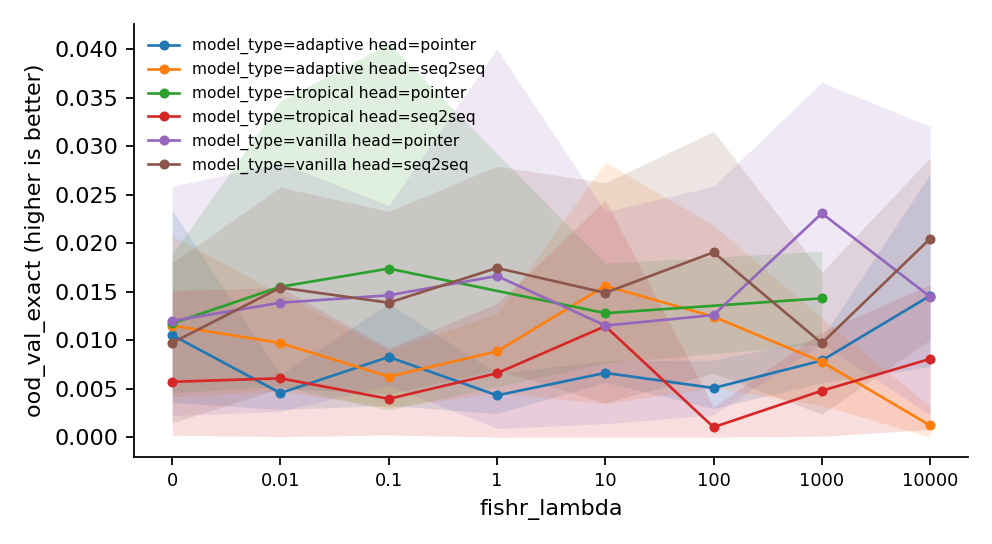
\includegraphics[width=\textwidth]{metric_ood_val_exact.png}
\caption{\texttt{ood\_val\_exact} against \texttt{fishr\_lambda}: the mean over seeds with a 95\% bootstrap CI, one line per combination of the other factors.}
\label{fig:ood_val_exact}
\end{figure}

{\small
\begin{longtable}{lllrlrrr}
\caption{\texttt{ood\_val\_exact} per cell: mean, 95\% bootstrap CI, SD, seeds, diverged runs.}\label{tab:summary-ood_val_exact}\\
\toprule
\texttt{model\_type} & \texttt{head} & \texttt{fishr\_lambda} & mean & 95\% CI & SD & $n$ & div.\\
\midrule
\endhead
adaptive & pointer & 0 & 0.01054 & [0.0036, 0.0234] & 0.0143 & 5 & 0\\
adaptive & pointer & 0.01 & 0.00456 & [0.00286, 0.00646] & 0.00235 & 5 & 0\\
adaptive & pointer & 0.1 & 0.00828 & [0.00328, 0.0138] & 0.00668 & 5 & 0\\
adaptive & pointer & 1 & 0.00432 & [0.00244, 0.0066] & 0.00267 & 5 & 0\\
adaptive & pointer & 10 & 0.00664 & [0.00566, 0.00786] & 0.00146 & 5 & 0\\
adaptive & pointer & 100 & 0.00508 & [0.00296, 0.00796] & 0.00316 & 5 & 0\\
adaptive & pointer & 1000 & 0.00792 & [0.00562, 0.0102] & 0.00298 & 5 & 0\\
adaptive & pointer & 1e+04 & 0.0146 & [0.00728, 0.0272] & 0.0137 & 5 & 0\\
adaptive & seq2seq & 0 & 0.01152 & [0.00418, 0.0208] & 0.011 & 5 & 0\\
adaptive & seq2seq & 0.01 & 0.00972 & [0.00478, 0.0148] & 0.00655 & 5 & 0\\
adaptive & seq2seq & 0.1 & 0.00626 & [0.00308, 0.00898] & 0.00388 & 5 & 0\\
adaptive & seq2seq & 1 & 0.00886 & [0.00456, 0.0127] & 0.00551 & 5 & 0\\
adaptive & seq2seq & 10 & 0.01562 & [0.00348, 0.0284] & 0.016 & 5 & 0\\
adaptive & seq2seq & 100 & 0.01244 & [0.0051, 0.0219] & 0.0111 & 5 & 0\\
adaptive & seq2seq & 1000 & 0.00778 & [0.00328, 0.0123] & 0.00606 & 5 & 0\\
adaptive & seq2seq & 1e+04 & 0.00122 & [$2.00\times10^{-5}$, 0.0032] & 0.00215 & 5 & 0\\
tropical & pointer & 0 & 0.01174 & [0.0046, 0.0189] & 0.00939 & 5 & 0\\
tropical & pointer & 0.01 & 0.01553 & [0.00525, 0.0347] & 0.0191 & 4 & 0\\
tropical & pointer & 0.1 & 0.0174 & [0.0028, 0.0406] & 0.0233 & 4 & 0\\
tropical & pointer & 10 & 0.0128 & [0.00765, 0.018] & 0.00638 & 4 & 0\\
tropical & pointer & 1000 & 0.01433 & [0.0096, 0.0192] & 0.0048 & 3 & 0\\
tropical & seq2seq & 0 & 0.00572 & [$2.20\times10^{-4}$, 0.0151] & 0.0103 & 5 & 0\\
tropical & seq2seq & 0.01 & 0.00608 & [$6.00\times10^{-5}$, 0.0155] & 0.0102 & 5 & 0\\
tropical & seq2seq & 0.1 & 0.00396 & [$2.40\times10^{-4}$, 0.00916] & 0.00576 & 5 & 0\\
tropical & seq2seq & 1 & 0.0066 & [0, 0.0138] & 0.0091 & 5 & 0\\
tropical & seq2seq & 10 & 0.01146 & [0, 0.0245] & 0.0159 & 5 & 0\\
tropical & seq2seq & 100 & 0.00104 & [0, 0.00312] & 0.00233 & 5 & 0\\
tropical & seq2seq & 1000 & 0.0048 & [$1.00\times10^{-4}$, 0.0109] & 0.00708 & 5 & 0\\
tropical & seq2seq & 1e+04 & 0.00808 & [$8.00\times10^{-4}$, 0.0158] & 0.00962 & 5 & 0\\
vanilla & pointer & 0 & 0.012 & [0.00224, 0.0259] & 0.0154 & 5 & 0\\
vanilla & pointer & 0.01 & 0.01388 & [0.00266, 0.0283] & 0.0159 & 5 & 0\\
vanilla & pointer & 0.1 & 0.01464 & [0.00536, 0.0239] & 0.0121 & 5 & 0\\
vanilla & pointer & 1 & 0.01664 & [$9.00\times10^{-4}$, 0.0401] & 0.0255 & 5 & 0\\
vanilla & pointer & 10 & 0.01152 & [0.0014, 0.0233] & 0.0141 & 5 & 0\\
vanilla & pointer & 100 & 0.0126 & [0.00232, 0.0259] & 0.0152 & 5 & 0\\
vanilla & pointer & 1000 & 0.0231 & [0.00962, 0.0366] & 0.0174 & 5 & 0\\
vanilla & pointer & 1e+04 & 0.0145 & [0.00232, 0.0321] & 0.0195 & 5 & 0\\
vanilla & seq2seq & 0 & 0.00974 & [0.00148, 0.018] & 0.0108 & 5 & 0\\
vanilla & seq2seq & 0.01 & 0.01544 & [0.00508, 0.0258] & 0.0133 & 5 & 0\\
vanilla & seq2seq & 0.1 & 0.01388 & [0.00446, 0.0233] & 0.0128 & 5 & 0\\
vanilla & seq2seq & 1 & 0.01746 & [0.00696, 0.028] & 0.0135 & 5 & 0\\
vanilla & seq2seq & 10 & 0.0149 & [0.00354, 0.0263] & 0.0143 & 5 & 0\\
vanilla & seq2seq & 100 & 0.01908 & [0.0066, 0.0316] & 0.0169 & 5 & 0\\
vanilla & seq2seq & 1000 & 0.0097 & [0.00238, 0.017] & 0.00929 & 5 & 0\\
vanilla & seq2seq & 1e+04 & 0.02048 & [0.01, 0.0288] & 0.0127 & 5 & 0\\
\bottomrule
\end{longtable}
}

{\small
\begin{longtable}{lllrrrl}
\caption{\texttt{ood\_val\_exact}: each level of \texttt{fishr\_lambda} against its control (0), within each combination of the other factors. rank: Wilcoxon signed-rank by seed, Holm.}\label{tab:control-ood_val_exact}\\
\toprule
\texttt{model\_type} & \texttt{head} & \texttt{fishr\_lambda} & difference & 95\% CI & $p$ & \\
\midrule
\endhead
adaptive & pointer & 0.01 & $-6.000\times10^{-4}$ & [-0.0193, 0.0019] & 1.0000 & \\
adaptive & pointer & 0.1 & $2.000\times10^{-4}$ & [-0.0177, 0.00936] & 1.0000 & \\
adaptive & pointer & 1 & 0 & [-0.0193, 0.00172] & 1.0000 & \\
adaptive & pointer & 10 & 0.0017 & [-0.0174, 0.00402] & 1.0000 & \\
adaptive & pointer & 100 & $-6.000\times10^{-4}$ & [-0.0182, 0.00262] & 1.0000 & \\
adaptive & pointer & 1000 & 0.0016 & [-0.0153, 0.00526] & 1.0000 & \\
adaptive & pointer & 1e+04 & 0.0027 & [0.00262, 0.00674] & 0.4375 & \\
adaptive & seq2seq & 0.01 & -0.0019 & [-0.00628, 0.0023] & 1.0000 & \\
adaptive & seq2seq & 0.1 & -0.003 & [-0.0127, 0.00102] & 1.0000 & \\
adaptive & seq2seq & 1 & $-1.000\times10^{-4}$ & [-0.01, 0.00354] & 1.0000 & \\
adaptive & seq2seq & 10 & $-5.000\times10^{-4}$ & [-0.00382, 0.0153] & 1.0000 & \\
adaptive & seq2seq & 100 & $7.000\times10^{-4}$ & [-0.00854, 0.0127] & 1.0000 & \\
adaptive & seq2seq & 1000 & $-3.000\times10^{-4}$ & [-0.017, 0.00478] & 1.0000 & \\
adaptive & seq2seq & 1e+04 & -0.0047 & [-0.0207, -0.00306] & 0.4375 & \\
tropical & pointer & 0.01 & -0.0042 & [-0.0153, 0.0222] & 1.0000 & \\
tropical & pointer & 0.1 & -0.00595 & [-0.0123, 0.0285] & 1.0000 & \\
tropical & pointer & 10 & -0.00125 & [-0.00775, 0.0107] & 1.0000 & \\
tropical & pointer & 1000 & -0.0091 & [-0.0094, 0.0127] & 1.0000 & \\
tropical & seq2seq & 0.01 & 0 & [-0.0105, 0.0119] & 1.0000 & \\
tropical & seq2seq & 0.1 & 0 & [-0.0112, 0.00598] & 1.0000 & \\
tropical & seq2seq & 1 & 0 & [-0.0036, 0.00668] & 1.0000 & \\
tropical & seq2seq & 10 & 0 & [$-6.60\times10^{-4}$, 0.0174] & 1.0000 & \\
tropical & seq2seq & 100 & 0 & [-0.0144, $8.00\times10^{-4}$] & 1.0000 & \\
tropical & seq2seq & 1000 & 0 & [-0.00992, 0.0075] & 1.0000 & \\
tropical & seq2seq & 1e+04 & 0 & [-0.00412, 0.0106] & 1.0000 & \\
vanilla & pointer & 0.01 & $5.000\times10^{-4}$ & [-0.00908, 0.0146] & 1.0000 & \\
vanilla & pointer & 0.1 & 0 & [-0.00918, 0.0146] & 1.0000 & \\
vanilla & pointer & 1 & -0.0012 & [-0.0109, 0.0268] & 1.0000 & \\
vanilla & pointer & 10 & $-5.000\times10^{-4}$ & [-0.00952, 0.00988] & 1.0000 & \\
vanilla & pointer & 100 & $3.000\times10^{-4}$ & [-0.0121, 0.0138] & 1.0000 & \\
vanilla & pointer & 1000 & 0.0058 & [0.0028, 0.0214] & 0.4375 & \\
vanilla & pointer & 1e+04 & 0.001 & [$6.00\times10^{-5}$, 0.00606] & 1.0000 & \\
vanilla & seq2seq & 0.01 & 0.0011 & [-0.00124, 0.0152] & 1.0000 & \\
vanilla & seq2seq & 0.1 & $-6.000\times10^{-4}$ & [-0.00188, 0.0114] & 1.0000 & \\
vanilla & seq2seq & 1 & 0.0067 & [$-9.80\times10^{-4}$, 0.0194] & 1.0000 & \\
vanilla & seq2seq & 10 & -0.0013 & [-0.0124, 0.0227] & 1.0000 & \\
vanilla & seq2seq & 100 & 0.0091 & [$5.00\times10^{-4}$, 0.0207] & 1.0000 & \\
vanilla & seq2seq & 1000 & -0.0038 & [-0.0116, 0.0127] & 1.0000 & \\
vanilla & seq2seq & 1e+04 & 0.004 & [$5.20\times10^{-4}$, 0.0237] & 1.0000 & \\
\bottomrule
\end{longtable}
}

{\small
\begin{longtable}{llrrrrr}
\caption{\texttt{ood\_val\_exact} against log10 \texttt{fishr\_lambda}: rank: Spearman rho, seed-bootstrap CI, with the Jonckheere--Terpstra ordered-trend $\tau$ and $p$.}\label{tab:trend-ood_val_exact}\\
\toprule
\texttt{model\_type} & \texttt{head} & estimate & 95\% CI & $p$ & JT $\tau$ & JT $p$\\
\midrule
\endhead
adaptive & pointer & 0.4089 & [0.0439, 0.721] & 0.0147 & 0.33 & 0.0138\\
adaptive & seq2seq & -0.3049 & [-0.54, 0.0384] & 0.0749 & -0.24 & 0.0640\\
tropical & pointer & 0.3132 & [-0.199, 0.855] & 0.2556 & 0.262 & 0.2877\\
tropical & seq2seq & -0.02856 & [-0.0731, 0.0398] & 0.8706 & -0.0152 & 0.9084\\
vanilla & pointer & 0.09411 & [-0.123, 0.399] & 0.5908 & 0.0762 & 0.5677\\
vanilla & seq2seq & $-7.083\times10^{-4}$ & [-0.294, 0.297] & 0.9968 & 0.0019 & 0.9964\\
\bottomrule
\end{longtable}
}

{\small
\begin{longtable}{lrrrl}
\caption{\texttt{ood\_val\_exact}: paired contrasts by seed, Holm-corrected across the cells. rank: Wilcoxon signed-rank by seed, Holm.}\label{tab:paired-ood_val_exact}\\
\toprule
contrast (within) & difference & 95\% CI & $p$ & \\
\midrule
\endhead
\stackcell{model\_type: tropical - vanilla\\\footnotesize head=pointer fishr\_lambda=0 } & $-2.600\times10^{-4}$ & [-0.0267, 0.0262] & 1.0000 & \\
\stackcell{model\_type: tropical - vanilla\\\footnotesize head=pointer fishr\_lambda=0.01 } & -0.00175 & [-0.0506, 0.0471] & 1.0000 & \\
\stackcell{model\_type: tropical - vanilla\\\footnotesize head=pointer fishr\_lambda=0.1 } & $-5.750\times10^{-4}$ & [-0.0371, 0.0359] & 1.0000 & \\
\stackcell{model\_type: tropical - vanilla\\\footnotesize head=pointer fishr\_lambda=10 } & -0.001025 & [-0.0151, 0.0131] & 1.0000 & \\
\stackcell{model\_type: tropical - vanilla\\\footnotesize head=pointer fishr\_lambda=1000 } & -0.008633 & [-0.0553, 0.038] & 1.0000 & \\
\stackcell{model\_type: tropical - vanilla\\\footnotesize head=seq2seq fishr\_lambda=0 } & -0.00402 & [-0.0141, 0.00608] & 1.0000 & \\
\stackcell{model\_type: tropical - vanilla\\\footnotesize head=seq2seq fishr\_lambda=0.01 } & -0.00936 & [-0.0215, 0.00276] & 0.8125 & \\
\stackcell{model\_type: tropical - vanilla\\\footnotesize head=seq2seq fishr\_lambda=0.1 } & -0.00992 & [-0.02, $1.28\times10^{-4}$] & 0.8125 & \\
\stackcell{model\_type: tropical - vanilla\\\footnotesize head=seq2seq fishr\_lambda=1 } & -0.01086 & [-0.0269, 0.00518] & 0.8125 & \\
\stackcell{model\_type: tropical - vanilla\\\footnotesize head=seq2seq fishr\_lambda=10 } & -0.00344 & [-0.0358, 0.0289] & 1.0000 & \\
\stackcell{model\_type: tropical - vanilla\\\footnotesize head=seq2seq fishr\_lambda=100 } & -0.01804 & [-0.0381, 0.002] & 1.0000 & \\
\stackcell{model\_type: tropical - vanilla\\\footnotesize head=seq2seq fishr\_lambda=1000 } & -0.0049 & [-0.0182, 0.00835] & 1.0000 & \\
\stackcell{model\_type: tropical - vanilla\\\footnotesize head=seq2seq fishr\_lambda=1e+04 } & -0.0124 & [-0.0288, 0.00399] & 1.0000 & \\
\stackcell{model\_type: adaptive - vanilla\\\footnotesize head=pointer fishr\_lambda=0 } & -0.00146 & [-0.0313, 0.0284] & 1.0000 & \\
\stackcell{model\_type: adaptive - vanilla\\\footnotesize head=pointer fishr\_lambda=0.01 } & -0.00932 & [-0.0278, 0.0092] & 1.0000 & \\
\stackcell{model\_type: adaptive - vanilla\\\footnotesize head=pointer fishr\_lambda=0.1 } & -0.00636 & [-0.0173, 0.00459] & 1.0000 & \\
\stackcell{model\_type: adaptive - vanilla\\\footnotesize head=pointer fishr\_lambda=1 } & -0.01232 & [-0.0412, 0.0166] & 1.0000 & \\
\stackcell{model\_type: adaptive - vanilla\\\footnotesize head=pointer fishr\_lambda=10 } & -0.00488 & [-0.0211, 0.0113] & 1.0000 & \\
\stackcell{model\_type: adaptive - vanilla\\\footnotesize head=pointer fishr\_lambda=100 } & -0.00752 & [-0.0233, 0.00829] & 1.0000 & \\
\stackcell{model\_type: adaptive - vanilla\\\footnotesize head=pointer fishr\_lambda=1000 } & -0.01518 & [-0.0361, 0.00578] & 1.0000 & \\
\stackcell{model\_type: adaptive - vanilla\\\footnotesize head=pointer fishr\_lambda=1e+04 } & $1.000\times10^{-4}$ & [-0.0309, 0.0311] & 1.0000 & \\
\stackcell{model\_type: adaptive - vanilla\\\footnotesize head=seq2seq fishr\_lambda=0 } & 0.00178 & [-0.0209, 0.0245] & 1.0000 & \\
\stackcell{model\_type: adaptive - vanilla\\\footnotesize head=seq2seq fishr\_lambda=0.01 } & -0.00572 & [-0.0206, 0.00913] & 1.0000 & \\
\stackcell{model\_type: adaptive - vanilla\\\footnotesize head=seq2seq fishr\_lambda=0.1 } & -0.00762 & [-0.0228, 0.00757] & 1.0000 & \\
\stackcell{model\_type: adaptive - vanilla\\\footnotesize head=seq2seq fishr\_lambda=1 } & -0.0086 & [-0.0189, 0.00172] & 1.0000 & \\
\stackcell{model\_type: adaptive - vanilla\\\footnotesize head=seq2seq fishr\_lambda=10 } & $7.200\times10^{-4}$ & [-0.00487, 0.00631] & 1.0000 & \\
\stackcell{model\_type: adaptive - vanilla\\\footnotesize head=seq2seq fishr\_lambda=100 } & -0.00664 & [-0.037, 0.0237] & 1.0000 & \\
\stackcell{model\_type: adaptive - vanilla\\\footnotesize head=seq2seq fishr\_lambda=1000 } & -0.00192 & [-0.0178, 0.014] & 1.0000 & \\
\stackcell{model\_type: adaptive - vanilla\\\footnotesize head=seq2seq fishr\_lambda=1e+04 } & -0.01926 & [-0.0375, $-9.90\times10^{-4}$] & 1.0000 & \\
\stackcell{head: pointer - seq2seq\\\footnotesize model\_type=adaptive fishr\_lambda=0 } & $-9.800\times10^{-4}$ & [-0.0281, 0.0261] & 1.0000 & \\
\stackcell{head: pointer - seq2seq\\\footnotesize model\_type=adaptive fishr\_lambda=0.01 } & -0.00516 & [-0.0155, 0.00514] & 1.0000 & \\
\stackcell{head: pointer - seq2seq\\\footnotesize model\_type=adaptive fishr\_lambda=0.1 } & 0.00202 & [-0.00558, 0.00962] & 1.0000 & \\
\stackcell{head: pointer - seq2seq\\\footnotesize model\_type=adaptive fishr\_lambda=1 } & -0.00454 & [-0.0128, 0.00372] & 1.0000 & \\
\stackcell{head: pointer - seq2seq\\\footnotesize model\_type=adaptive fishr\_lambda=10 } & -0.00898 & [-0.0296, 0.0116] & 1.0000 & \\
\stackcell{head: pointer - seq2seq\\\footnotesize model\_type=adaptive fishr\_lambda=100 } & -0.00736 & [-0.0235, 0.0088] & 1.0000 & \\
\stackcell{head: pointer - seq2seq\\\footnotesize model\_type=adaptive fishr\_lambda=1000 } & $1.400\times10^{-4}$ & [-0.00937, 0.00965] & 1.0000 & \\
\stackcell{head: pointer - seq2seq\\\footnotesize model\_type=adaptive fishr\_lambda=1e+04 } & 0.01338 & [-0.00427, 0.031] & 1.0000 & \\
\stackcell{head: pointer - seq2seq\\\footnotesize model\_type=tropical fishr\_lambda=0 } & 0.00602 & [-0.00703, 0.0191] & 1.0000 & \\
\stackcell{head: pointer - seq2seq\\\footnotesize model\_type=tropical fishr\_lambda=0.01 } & 0.01383 & [-0.019, 0.0467] & 1.0000 & \\
\stackcell{head: pointer - seq2seq\\\footnotesize model\_type=tropical fishr\_lambda=0.1 } & 0.01582 & [-0.0228, 0.0545] & 1.0000 & \\
\stackcell{head: pointer - seq2seq\\\footnotesize model\_type=tropical fishr\_lambda=10 } & -0.001525 & [-0.038, 0.035] & 1.0000 & \\
\stackcell{head: pointer - seq2seq\\\footnotesize model\_type=tropical fishr\_lambda=1000 } & 0.0065 & [-0.0101, 0.0231] & 1.0000 & \\
\stackcell{head: pointer - seq2seq\\\footnotesize model\_type=vanilla fishr\_lambda=0 } & 0.00226 & [-0.0257, 0.0302] & 1.0000 & \\
\stackcell{head: pointer - seq2seq\\\footnotesize model\_type=vanilla fishr\_lambda=0.01 } & -0.00156 & [-0.0371, 0.034] & 1.0000 & \\
\stackcell{head: pointer - seq2seq\\\footnotesize model\_type=vanilla fishr\_lambda=0.1 } & $7.600\times10^{-4}$ & [-0.0268, 0.0283] & 1.0000 & \\
\stackcell{head: pointer - seq2seq\\\footnotesize model\_type=vanilla fishr\_lambda=1 } & $-8.200\times10^{-4}$ & [-0.0455, 0.0439] & 1.0000 & \\
\stackcell{head: pointer - seq2seq\\\footnotesize model\_type=vanilla fishr\_lambda=10 } & -0.00338 & [-0.0245, 0.0177] & 1.0000 & \\
\stackcell{head: pointer - seq2seq\\\footnotesize model\_type=vanilla fishr\_lambda=100 } & -0.00648 & [-0.045, 0.032] & 1.0000 & \\
\stackcell{head: pointer - seq2seq\\\footnotesize model\_type=vanilla fishr\_lambda=1000 } & 0.0134 & [-0.00896, 0.0358] & 1.0000 & \\
\stackcell{head: pointer - seq2seq\\\footnotesize model\_type=vanilla fishr\_lambda=1e+04 } & -0.00598 & [-0.0456, 0.0336] & 1.0000 & \\
\bottomrule
\end{longtable}
}

\subsection{\texttt{ood\_noise\_f1}}
\begin{figure}[tbp]
\centering
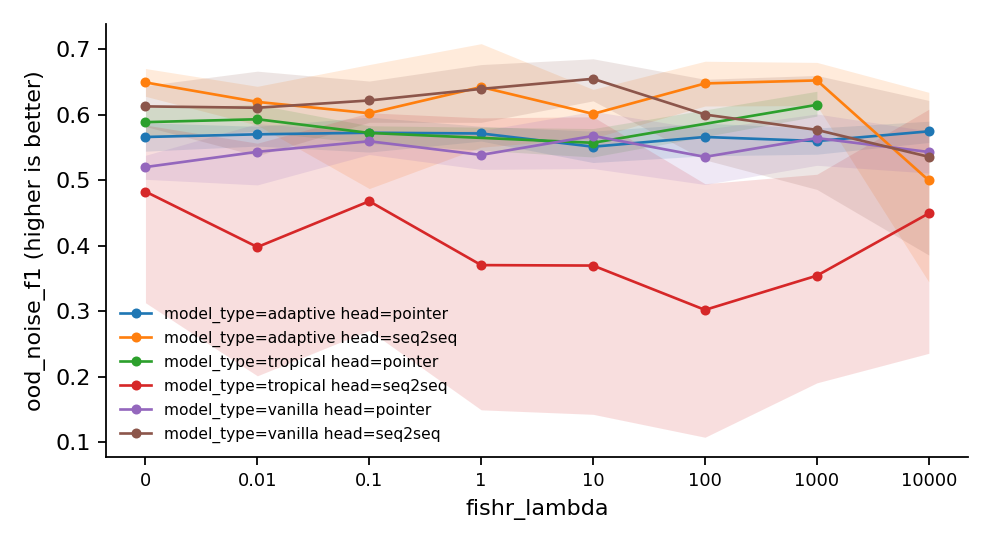
\includegraphics[width=\textwidth]{metric_ood_noise_f1.png}
\caption{\texttt{ood\_noise\_f1} against \texttt{fishr\_lambda}: the mean over seeds with a 95\% bootstrap CI, one line per combination of the other factors.}
\label{fig:ood_noise_f1}
\end{figure}

{\small
\begin{longtable}{lllrlrrr}
\caption{\texttt{ood\_noise\_f1} per cell: mean, 95\% bootstrap CI, SD, seeds, diverged runs.}\label{tab:summary-ood_noise_f1}\\
\toprule
\texttt{model\_type} & \texttt{head} & \texttt{fishr\_lambda} & mean & 95\% CI & SD & $n$ & div.\\
\midrule
\endhead
adaptive & pointer & 0 & 0.5657 & [0.544, 0.588] & 0.0287 & 5 & 0\\
adaptive & pointer & 0.01 & 0.5698 & [0.552, 0.582] & 0.0201 & 5 & 0\\
adaptive & pointer & 0.1 & 0.5722 & [0.543, 0.596] & 0.0343 & 5 & 0\\
adaptive & pointer & 1 & 0.5711 & [0.559, 0.582] & 0.0146 & 5 & 0\\
adaptive & pointer & 10 & 0.5509 & [0.527, 0.575] & 0.0327 & 5 & 0\\
adaptive & pointer & 100 & 0.5657 & [0.537, 0.587] & 0.033 & 5 & 0\\
adaptive & pointer & 1000 & 0.5595 & [0.539, 0.579] & 0.0252 & 5 & 0\\
adaptive & pointer & 1e+04 & 0.5743 & [0.557, 0.59] & 0.0209 & 5 & 0\\
adaptive & seq2seq & 0 & 0.649 & [0.628, 0.67] & 0.0275 & 5 & 0\\
adaptive & seq2seq & 0.01 & 0.6193 & [0.584, 0.643] & 0.0407 & 5 & 0\\
adaptive & seq2seq & 0.1 & 0.602 & [0.487, 0.676] & 0.128 & 5 & 0\\
adaptive & seq2seq & 1 & 0.642 & [0.55, 0.708] & 0.107 & 5 & 0\\
adaptive & seq2seq & 10 & 0.601 & [0.564, 0.638] & 0.0469 & 5 & 0\\
adaptive & seq2seq & 100 & 0.6475 & [0.613, 0.681] & 0.0464 & 5 & 0\\
adaptive & seq2seq & 1000 & 0.6521 & [0.614, 0.68] & 0.0446 & 5 & 0\\
adaptive & seq2seq & 1e+04 & 0.4993 & [0.344, 0.634] & 0.195 & 5 & 0\\
tropical & pointer & 0 & 0.5883 & [0.566, 0.61] & 0.0295 & 5 & 0\\
tropical & pointer & 0.01 & 0.5928 & [0.574, 0.615] & 0.0241 & 4 & 0\\
tropical & pointer & 0.1 & 0.5719 & [0.556, 0.583] & 0.0163 & 4 & 0\\
tropical & pointer & 10 & 0.5568 & [0.535, 0.579] & 0.0262 & 4 & 0\\
tropical & pointer & 1000 & 0.6148 & [0.598, 0.636] & 0.0192 & 3 & 0\\
tropical & seq2seq & 0 & 0.4824 & [0.313, 0.584] & 0.189 & 5 & 0\\
tropical & seq2seq & 0.01 & 0.3977 & [0.201, 0.556] & 0.217 & 5 & 0\\
tropical & seq2seq & 0.1 & 0.4676 & [0.27, 0.603] & 0.223 & 5 & 0\\
tropical & seq2seq & 1 & 0.3701 & [0.149, 0.595] & 0.293 & 5 & 0\\
tropical & seq2seq & 10 & 0.3694 & [0.142, 0.597] & 0.289 & 5 & 0\\
tropical & seq2seq & 100 & 0.3017 & [0.107, 0.494] & 0.254 & 5 & 0\\
tropical & seq2seq & 1000 & 0.354 & [0.19, 0.509] & 0.218 & 5 & 0\\
tropical & seq2seq & 1e+04 & 0.4491 & [0.235, 0.608] & 0.248 & 5 & 0\\
vanilla & pointer & 0 & 0.5198 & [0.501, 0.538] & 0.0239 & 5 & 0\\
vanilla & pointer & 0.01 & 0.5431 & [0.493, 0.586] & 0.0603 & 5 & 0\\
vanilla & pointer & 0.1 & 0.5592 & [0.539, 0.572] & 0.0228 & 5 & 0\\
vanilla & pointer & 1 & 0.5383 & [0.516, 0.575] & 0.0387 & 5 & 0\\
vanilla & pointer & 10 & 0.5674 & [0.518, 0.605] & 0.058 & 5 & 0\\
vanilla & pointer & 100 & 0.5353 & [0.493, 0.578] & 0.055 & 5 & 0\\
vanilla & pointer & 1000 & 0.564 & [0.522, 0.601] & 0.0501 & 5 & 0\\
vanilla & pointer & 1e+04 & 0.5428 & [0.511, 0.575] & 0.0422 & 5 & 0\\
vanilla & seq2seq & 0 & 0.6124 & [0.582, 0.644] & 0.0403 & 5 & 0\\
vanilla & seq2seq & 0.01 & 0.6103 & [0.537, 0.666] & 0.0836 & 5 & 0\\
vanilla & seq2seq & 0.1 & 0.6215 & [0.588, 0.651] & 0.0408 & 5 & 0\\
vanilla & seq2seq & 1 & 0.6391 & [0.588, 0.676] & 0.0563 & 5 & 0\\
vanilla & seq2seq & 10 & 0.6545 & [0.621, 0.685] & 0.0435 & 5 & 0\\
vanilla & seq2seq & 100 & 0.5999 & [0.531, 0.654] & 0.0817 & 5 & 0\\
vanilla & seq2seq & 1000 & 0.5765 & [0.486, 0.66] & 0.109 & 5 & 0\\
vanilla & seq2seq & 1e+04 & 0.5354 & [0.385, 0.622] & 0.165 & 5 & 0\\
\bottomrule
\end{longtable}
}

{\small
\begin{longtable}{lllrrrl}
\caption{\texttt{ood\_noise\_f1}: each level of \texttt{fishr\_lambda} against its control (0), within each combination of the other factors. parametric: Dunnett vs control.}\label{tab:control-ood_noise_f1}\\
\toprule
\texttt{model\_type} & \texttt{head} & \texttt{fishr\_lambda} & difference & 95\% CI & $p$ & \\
\midrule
\endhead
adaptive & pointer & 0.01 & 0.004067 & [-0.0431, 0.0513] & 1.0000 & \\
adaptive & pointer & 0.1 & 0.00648 & [-0.0407, 0.0537] & 0.9991 & \\
adaptive & pointer & 1 & 0.00536 & [-0.0418, 0.0525] & 0.9997 & \\
adaptive & pointer & 10 & -0.01483 & [-0.062, 0.0324] & 0.9181 & \\
adaptive & pointer & 100 & $1.744\times10^{-5}$ & [-0.0472, 0.0472] & 1.0000 & \\
adaptive & pointer & 1000 & -0.006204 & [-0.0534, 0.041] & 0.9994 & \\
adaptive & pointer & 1e+04 & 0.008623 & [-0.0386, 0.0558] & 0.9951 & \\
adaptive & seq2seq & 0.01 & -0.02972 & [-0.198, 0.139] & 0.9961 & \\
adaptive & seq2seq & 0.1 & -0.04704 & [-0.216, 0.122] & 0.9526 & \\
adaptive & seq2seq & 1 & -0.007006 & [-0.176, 0.162] & 1.0000 & \\
adaptive & seq2seq & 10 & -0.04801 & [-0.217, 0.121] & 0.9478 & \\
adaptive & seq2seq & 100 & -0.001531 & [-0.17, 0.167] & 1.0000 & \\
adaptive & seq2seq & 1000 & 0.003071 & [-0.166, 0.172] & 1.0000 & \\
adaptive & seq2seq & 1e+04 & -0.1497 & [-0.318, 0.0191] & 0.0990 & \\
tropical & pointer & 0.01 & 0.004452 & [-0.0403, 0.0492] & 0.9964 & \\
tropical & pointer & 0.1 & -0.01647 & [-0.0612, 0.0283] & 0.7270 & \\
tropical & pointer & 10 & -0.03152 & [-0.0763, 0.0132] & 0.2157 & \\
tropical & pointer & 1000 & 0.02645 & [-0.0223, 0.0752] & 0.4214 & \\
tropical & seq2seq & 0.01 & -0.0847 & [-0.511, 0.341] & 0.9920 & \\
tropical & seq2seq & 0.1 & -0.01472 & [-0.441, 0.411] & 1.0000 & \\
tropical & seq2seq & 1 & -0.1123 & [-0.538, 0.314] & 0.9638 & \\
tropical & seq2seq & 10 & -0.113 & [-0.539, 0.313] & 0.9627 & \\
tropical & seq2seq & 100 & -0.1807 & [-0.606, 0.245] & 0.7479 & \\
tropical & seq2seq & 1000 & -0.1284 & [-0.554, 0.297] & 0.9319 & \\
tropical & seq2seq & 1e+04 & -0.03325 & [-0.459, 0.393] & 1.0000 & \\
vanilla & pointer & 0.01 & 0.02329 & [-0.057, 0.104] & 0.9428 & \\
vanilla & pointer & 0.1 & 0.03942 & [-0.0409, 0.12] & 0.6189 & \\
vanilla & pointer & 1 & 0.01856 & [-0.0617, 0.0988] & 0.9816 & \\
vanilla & pointer & 10 & 0.04759 & [-0.0327, 0.128] & 0.4283 & \\
vanilla & pointer & 100 & 0.01556 & [-0.0647, 0.0958] & 0.9931 & \\
vanilla & pointer & 1000 & 0.04425 & [-0.036, 0.125] & 0.5031 & \\
vanilla & pointer & 1e+04 & 0.02299 & [-0.0573, 0.103] & 0.9463 & \\
vanilla & seq2seq & 0.01 & -0.002057 & [-0.155, 0.151] & 1.0000 & \\
vanilla & seq2seq & 0.1 & 0.009067 & [-0.144, 0.162] & 1.0000 & \\
vanilla & seq2seq & 1 & 0.0267 & [-0.126, 0.179] & 0.9962 & \\
vanilla & seq2seq & 10 & 0.04212 & [-0.111, 0.195] & 0.9548 & \\
vanilla & seq2seq & 100 & -0.01249 & [-0.165, 0.14] & 1.0000 & \\
vanilla & seq2seq & 1000 & -0.03588 & [-0.189, 0.117] & 0.9799 & \\
vanilla & seq2seq & 1e+04 & -0.07696 & [-0.23, 0.0757] & 0.5932 & \\
\bottomrule
\end{longtable}
}

{\small
\begin{longtable}{llrrrrr}
\caption{\texttt{ood\_noise\_f1} against log10 \texttt{fishr\_lambda}: parametric: OLS slope t-test, seed-bootstrap CI, with the Jonckheere--Terpstra ordered-trend $\tau$ and $p$.}\label{tab:trend-ood_noise_f1}\\
\toprule
\texttt{model\_type} & \texttt{head} & estimate & 95\% CI & $p$ & JT $\tau$ & JT $p$\\
\midrule
\endhead
adaptive & pointer & $-6.086\times10^{-4}$ & [-0.00414, 0.00165] & 0.7825 & -0.0438 & 0.7530\\
adaptive & seq2seq & -0.009077 & [-0.0333, 0.011] & 0.3161 & -0.0476 & 0.7355\\
tropical & pointer & 0.002916 & [-0.00658, 0.00943] & 0.4973 & 0.0476 & 0.8868\\
tropical & seq2seq & -0.005046 & [-0.0232, 0.0131] & 0.8026 & -0.0324 & 0.8206\\
vanilla & pointer & $2.052\times10^{-4}$ & [-0.00625, 0.00666] & 0.9584 & 0.00571 & 0.9792\\
vanilla & seq2seq & -0.01264 & [-0.0271, -0.00182] & 0.1037 & -0.189 & 0.1682\\
\bottomrule
\end{longtable}
}

{\small
\begin{longtable}{lrrrl}
\caption{\texttt{ood\_noise\_f1}: paired contrasts by seed, Holm-corrected across the cells. parametric: paired t-test by seed, Holm.}\label{tab:paired-ood_noise_f1}\\
\toprule
contrast (within) & difference & 95\% CI & $p$ & \\
\midrule
\endhead
\stackcell{model\_type: tropical - vanilla\\\footnotesize head=pointer fishr\_lambda=0 } & 0.06857 & [0.0209, 0.116] & 0.2101 & \\
\stackcell{model\_type: tropical - vanilla\\\footnotesize head=pointer fishr\_lambda=0.01 } & 0.0616 & [-0.0606, 0.184] & 0.9910 & \\
\stackcell{model\_type: tropical - vanilla\\\footnotesize head=pointer fishr\_lambda=0.1 } & 0.01632 & [-0.0405, 0.0731] & 0.9910 & \\
\stackcell{model\_type: tropical - vanilla\\\footnotesize head=pointer fishr\_lambda=10 } & $-7.843\times10^{-4}$ & [-0.0902, 0.0886] & 0.9910 & \\
\stackcell{model\_type: tropical - vanilla\\\footnotesize head=pointer fishr\_lambda=1000 } & 0.0621 & [-0.0225, 0.147] & 0.7529 & \\
\stackcell{model\_type: tropical - vanilla\\\footnotesize head=seq2seq fishr\_lambda=0 } & -0.13 & [-0.385, 0.125] & 0.9910 & \\
\stackcell{model\_type: tropical - vanilla\\\footnotesize head=seq2seq fishr\_lambda=0.01 } & -0.2127 & [-0.383, -0.042] & 0.3100 & \\
\stackcell{model\_type: tropical - vanilla\\\footnotesize head=seq2seq fishr\_lambda=0.1 } & -0.1538 & [-0.406, 0.098] & 0.9910 & \\
\stackcell{model\_type: tropical - vanilla\\\footnotesize head=seq2seq fishr\_lambda=1 } & -0.269 & [-0.6, 0.0624] & 0.7529 & \\
\stackcell{model\_type: tropical - vanilla\\\footnotesize head=seq2seq fishr\_lambda=10 } & -0.2851 & [-0.63, 0.0598] & 0.7529 & \\
\stackcell{model\_type: tropical - vanilla\\\footnotesize head=seq2seq fishr\_lambda=100 } & -0.2982 & [-0.589, -0.00777] & 0.5100 & \\
\stackcell{model\_type: tropical - vanilla\\\footnotesize head=seq2seq fishr\_lambda=1000 } & -0.2225 & [-0.481, 0.0361] & 0.7529 & \\
\stackcell{model\_type: tropical - vanilla\\\footnotesize head=seq2seq fishr\_lambda=1e+04 } & -0.08633 & [-0.233, 0.06] & 0.9910 & \\
\stackcell{model\_type: adaptive - vanilla\\\footnotesize head=pointer fishr\_lambda=0 } & 0.04592 & [-0.00583, 0.0977] & 1.0000 & \\
\stackcell{model\_type: adaptive - vanilla\\\footnotesize head=pointer fishr\_lambda=0.01 } & 0.0267 & [-0.0617, 0.115] & 1.0000 & \\
\stackcell{model\_type: adaptive - vanilla\\\footnotesize head=pointer fishr\_lambda=0.1 } & 0.01298 & [-0.0499, 0.0758] & 1.0000 & \\
\stackcell{model\_type: adaptive - vanilla\\\footnotesize head=pointer fishr\_lambda=1 } & 0.03272 & [-0.0145, 0.0799] & 1.0000 & \\
\stackcell{model\_type: adaptive - vanilla\\\footnotesize head=pointer fishr\_lambda=10 } & -0.0165 & [-0.107, 0.0739] & 1.0000 & \\
\stackcell{model\_type: adaptive - vanilla\\\footnotesize head=pointer fishr\_lambda=100 } & 0.03037 & [-0.0266, 0.0873] & 1.0000 & \\
\stackcell{model\_type: adaptive - vanilla\\\footnotesize head=pointer fishr\_lambda=1000 } & -0.004534 & [-0.0766, 0.0676] & 1.0000 & \\
\stackcell{model\_type: adaptive - vanilla\\\footnotesize head=pointer fishr\_lambda=1e+04 } & 0.03156 & [-0.0172, 0.0803] & 1.0000 & \\
\stackcell{model\_type: adaptive - vanilla\\\footnotesize head=seq2seq fishr\_lambda=0 } & 0.03659 & [-0.0282, 0.101] & 1.0000 & \\
\stackcell{model\_type: adaptive - vanilla\\\footnotesize head=seq2seq fishr\_lambda=0.01 } & 0.00893 & [-0.104, 0.122] & 1.0000 & \\
\stackcell{model\_type: adaptive - vanilla\\\footnotesize head=seq2seq fishr\_lambda=0.1 } & -0.01951 & [-0.158, 0.119] & 1.0000 & \\
\stackcell{model\_type: adaptive - vanilla\\\footnotesize head=seq2seq fishr\_lambda=1 } & 0.002889 & [-0.0781, 0.0839] & 1.0000 & \\
\stackcell{model\_type: adaptive - vanilla\\\footnotesize head=seq2seq fishr\_lambda=10 } & -0.05354 & [-0.102, -0.00512] & 0.5968 & \\
\stackcell{model\_type: adaptive - vanilla\\\footnotesize head=seq2seq fishr\_lambda=100 } & 0.04755 & [-0.0951, 0.19] & 1.0000 & \\
\stackcell{model\_type: adaptive - vanilla\\\footnotesize head=seq2seq fishr\_lambda=1000 } & 0.07555 & [-0.0655, 0.217] & 1.0000 & \\
\stackcell{model\_type: adaptive - vanilla\\\footnotesize head=seq2seq fishr\_lambda=1e+04 } & -0.03612 & [-0.402, 0.329] & 1.0000 & \\
\stackcell{head: pointer - seq2seq\\\footnotesize model\_type=adaptive fishr\_lambda=0 } & -0.0833 & [-0.139, -0.0276] & 0.2705 & \\
\stackcell{head: pointer - seq2seq\\\footnotesize model\_type=adaptive fishr\_lambda=0.01 } & -0.04951 & [-0.108, 0.00943] & 1.0000 & \\
\stackcell{head: pointer - seq2seq\\\footnotesize model\_type=adaptive fishr\_lambda=0.1 } & -0.02979 & [-0.155, 0.0954] & 1.0000 & \\
\stackcell{head: pointer - seq2seq\\\footnotesize model\_type=adaptive fishr\_lambda=1 } & -0.07094 & [-0.204, 0.0621] & 1.0000 & \\
\stackcell{head: pointer - seq2seq\\\footnotesize model\_type=adaptive fishr\_lambda=10 } & -0.05013 & [-0.105, 0.00495] & 1.0000 & \\
\stackcell{head: pointer - seq2seq\\\footnotesize model\_type=adaptive fishr\_lambda=100 } & -0.08175 & [-0.174, 0.0107] & 1.0000 & \\
\stackcell{head: pointer - seq2seq\\\footnotesize model\_type=adaptive fishr\_lambda=1000 } & -0.09258 & [-0.149, -0.0364] & 0.2039 & \\
\stackcell{head: pointer - seq2seq\\\footnotesize model\_type=adaptive fishr\_lambda=1e+04 } & 0.07499 & [-0.185, 0.335] & 1.0000 & \\
\stackcell{head: pointer - seq2seq\\\footnotesize model\_type=tropical fishr\_lambda=0 } & 0.106 & [-0.109, 0.321] & 1.0000 & \\
\stackcell{head: pointer - seq2seq\\\footnotesize model\_type=tropical fishr\_lambda=0.01 } & 0.2565 & [-0.0283, 0.541] & 1.0000 & \\
\stackcell{head: pointer - seq2seq\\\footnotesize model\_type=tropical fishr\_lambda=0.1 } & 0.1439 & [-0.207, 0.494] & 1.0000 & \\
\stackcell{head: pointer - seq2seq\\\footnotesize model\_type=tropical fishr\_lambda=10 } & 0.1351 & [-0.33, 0.6] & 1.0000 & \\
\stackcell{head: pointer - seq2seq\\\footnotesize model\_type=tropical fishr\_lambda=1000 } & 0.2268 & [-0.509, 0.963] & 1.0000 & \\
\stackcell{head: pointer - seq2seq\\\footnotesize model\_type=vanilla fishr\_lambda=0 } & -0.09263 & [-0.143, -0.0426] & 0.1428 & \\
\stackcell{head: pointer - seq2seq\\\footnotesize model\_type=vanilla fishr\_lambda=0.01 } & -0.06728 & [-0.208, 0.0735] & 1.0000 & \\
\stackcell{head: pointer - seq2seq\\\footnotesize model\_type=vanilla fishr\_lambda=0.1 } & -0.06227 & [-0.129, 0.00396] & 1.0000 & \\
\stackcell{head: pointer - seq2seq\\\footnotesize model\_type=vanilla fishr\_lambda=1 } & -0.1008 & [-0.187, -0.0144] & 0.5715 & \\
\stackcell{head: pointer - seq2seq\\\footnotesize model\_type=vanilla fishr\_lambda=10 } & -0.08716 & [-0.193, 0.0187] & 1.0000 & \\
\stackcell{head: pointer - seq2seq\\\footnotesize model\_type=vanilla fishr\_lambda=100 } & -0.06457 & [-0.149, 0.0194] & 1.0000 & \\
\stackcell{head: pointer - seq2seq\\\footnotesize model\_type=vanilla fishr\_lambda=1000 } & -0.0125 & [-0.143, 0.118] & 1.0000 & \\
\stackcell{head: pointer - seq2seq\\\footnotesize model\_type=vanilla fishr\_lambda=1e+04 } & 0.007316 & [-0.185, 0.199] & 1.0000 & \\
\bottomrule
\end{longtable}
}

\subsection{\texttt{ood\_noise\_exact}}
\begin{figure}[tbp]
\centering
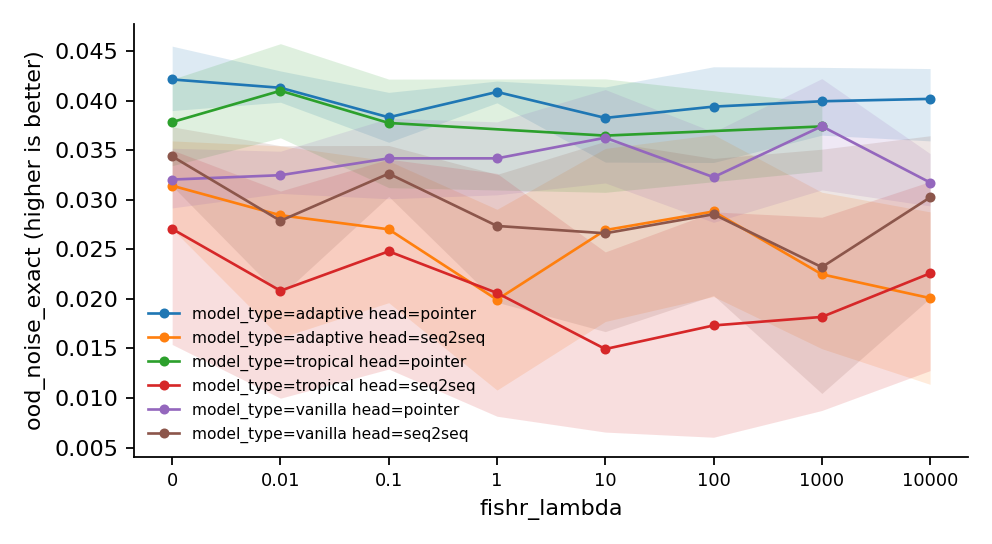
\includegraphics[width=\textwidth]{metric_ood_noise_exact.png}
\caption{\texttt{ood\_noise\_exact} against \texttt{fishr\_lambda}: the mean over seeds with a 95\% bootstrap CI, one line per combination of the other factors.}
\label{fig:ood_noise_exact}
\end{figure}

{\small
\begin{longtable}{lllrlrrr}
\caption{\texttt{ood\_noise\_exact} per cell: mean, 95\% bootstrap CI, SD, seeds, diverged runs.}\label{tab:summary-ood_noise_exact}\\
\toprule
\texttt{model\_type} & \texttt{head} & \texttt{fishr\_lambda} & mean & 95\% CI & SD & $n$ & div.\\
\midrule
\endhead
adaptive & pointer & 0 & 0.04214 & [0.039, 0.0455] & 0.00391 & 5 & 0\\
adaptive & pointer & 0.01 & 0.0413 & [0.0398, 0.043] & 0.00205 & 5 & 0\\
adaptive & pointer & 0.1 & 0.03832 & [0.0358, 0.0408] & 0.00331 & 5 & 0\\
adaptive & pointer & 1 & 0.04088 & [0.0398, 0.042] & 0.00143 & 5 & 0\\
adaptive & pointer & 10 & 0.03826 & [0.0338, 0.0414] & 0.00508 & 5 & 0\\
adaptive & pointer & 100 & 0.0394 & [0.0338, 0.0434] & 0.00638 & 5 & 0\\
adaptive & pointer & 1000 & 0.03994 & [0.0365, 0.0434] & 0.00457 & 5 & 0\\
adaptive & pointer & 1e+04 & 0.04018 & [0.0359, 0.0432] & 0.0048 & 5 & 0\\
adaptive & seq2seq & 0 & 0.03142 & [0.0271, 0.0359] & 0.00569 & 5 & 0\\
adaptive & seq2seq & 0.01 & 0.02844 & [0.0161, 0.0354] & 0.0136 & 5 & 0\\
adaptive & seq2seq & 0.1 & 0.02702 & [0.0196, 0.0339] & 0.00958 & 5 & 0\\
adaptive & seq2seq & 1 & 0.01992 & [0.0108, 0.029] & 0.0117 & 5 & 0\\
adaptive & seq2seq & 10 & 0.02694 & [0.0177, 0.0352] & 0.0117 & 5 & 0\\
adaptive & seq2seq & 100 & 0.02882 & [0.0202, 0.0366] & 0.0104 & 5 & 0\\
adaptive & seq2seq & 1000 & 0.02248 & [0.015, 0.0308] & 0.0101 & 5 & 0\\
adaptive & seq2seq & 1e+04 & 0.02008 & [0.0114, 0.0288] & 0.0114 & 5 & 0\\
tropical & pointer & 0 & 0.03784 & [0.0334, 0.0422] & 0.00533 & 5 & 0\\
tropical & pointer & 0.01 & 0.041 & [0.0363, 0.0457] & 0.00577 & 4 & 0\\
tropical & pointer & 0.1 & 0.03775 & [0.0312, 0.0422] & 0.00665 & 4 & 0\\
tropical & pointer & 10 & 0.03648 & [0.0307, 0.0422] & 0.00692 & 4 & 0\\
tropical & pointer & 1000 & 0.0374 & [0.0329, 0.0398] & 0.0039 & 3 & 0\\
tropical & seq2seq & 0 & 0.02706 & [0.0154, 0.035] & 0.013 & 5 & 0\\
tropical & seq2seq & 0.01 & 0.02082 & [0.00998, 0.0309] & 0.0133 & 5 & 0\\
tropical & seq2seq & 0.1 & 0.0248 & [0.0129, 0.0341] & 0.0137 & 5 & 0\\
tropical & seq2seq & 1 & 0.0206 & [0.00816, 0.0327] & 0.0161 & 5 & 0\\
tropical & seq2seq & 10 & 0.01494 & [0.00656, 0.0247] & 0.0115 & 5 & 0\\
tropical & seq2seq & 100 & 0.01732 & [0.00604, 0.0288] & 0.0148 & 5 & 0\\
tropical & seq2seq & 1000 & 0.01818 & [0.00874, 0.0282] & 0.0129 & 5 & 0\\
tropical & seq2seq & 1e+04 & 0.02258 & [0.0128, 0.0318] & 0.0129 & 5 & 0\\
vanilla & pointer & 0 & 0.03204 & [0.0292, 0.0352] & 0.00383 & 5 & 0\\
vanilla & pointer & 0.01 & 0.03248 & [0.0306, 0.0349] & 0.00279 & 5 & 0\\
vanilla & pointer & 0.1 & 0.03418 & [0.0301, 0.0382] & 0.00541 & 5 & 0\\
vanilla & pointer & 1 & 0.03418 & [0.0305, 0.0379] & 0.00468 & 5 & 0\\
vanilla & pointer & 10 & 0.03626 & [0.0317, 0.0411] & 0.0061 & 5 & 0\\
vanilla & pointer & 100 & 0.03228 & [0.0277, 0.0368] & 0.00599 & 5 & 0\\
vanilla & pointer & 1000 & 0.03742 & [0.031, 0.0422] & 0.00717 & 5 & 0\\
vanilla & pointer & 1e+04 & 0.03174 & [0.0294, 0.0347] & 0.00362 & 5 & 0\\
vanilla & seq2seq & 0 & 0.03438 & [0.0314, 0.0374] & 0.00418 & 5 & 0\\
vanilla & seq2seq & 0.01 & 0.02788 & [0.0203, 0.0355] & 0.00982 & 5 & 0\\
vanilla & seq2seq & 0.1 & 0.03264 & [0.0303, 0.0355] & 0.00331 & 5 & 0\\
vanilla & seq2seq & 1 & 0.02736 & [0.0197, 0.0326] & 0.00858 & 5 & 0\\
vanilla & seq2seq & 10 & 0.02662 & [0.0167, 0.0359] & 0.0135 & 5 & 0\\
vanilla & seq2seq & 100 & 0.02854 & [0.0203, 0.0342] & 0.00925 & 5 & 0\\
vanilla & seq2seq & 1000 & 0.0232 & [0.0105, 0.0351] & 0.0164 & 5 & 0\\
vanilla & seq2seq & 1e+04 & 0.03024 & [0.0201, 0.0365] & 0.0114 & 5 & 0\\
\bottomrule
\end{longtable}
}

{\small
\begin{longtable}{lllrrrl}
\caption{\texttt{ood\_noise\_exact}: each level of \texttt{fishr\_lambda} against its control (0), within each combination of the other factors. parametric: Dunnett vs control.}\label{tab:control-ood_noise_exact}\\
\toprule
\texttt{model\_type} & \texttt{head} & \texttt{fishr\_lambda} & difference & 95\% CI & $p$ & \\
\midrule
\endhead
adaptive & pointer & 0.01 & $-8.400\times10^{-4}$ & [-0.00822, 0.00654] & 0.9997 & \\
adaptive & pointer & 0.1 & -0.00382 & [-0.0112, 0.00356] & 0.5673 & \\
adaptive & pointer & 1 & -0.00126 & [-0.00864, 0.00612] & 0.9967 & \\
adaptive & pointer & 10 & -0.00388 & [-0.0113, 0.0035] & 0.5514 & \\
adaptive & pointer & 100 & -0.00274 & [-0.0101, 0.00464] & 0.8402 & \\
adaptive & pointer & 1000 & -0.0022 & [-0.00958, 0.00518] & 0.9353 & \\
adaptive & pointer & 1e+04 & -0.00196 & [-0.00934, 0.00542] & 0.9626 & \\
adaptive & seq2seq & 0.01 & -0.00298 & [-0.0218, 0.0158] & 0.9979 & \\
adaptive & seq2seq & 0.1 & -0.0044 & [-0.0232, 0.0144] & 0.9804 & \\
adaptive & seq2seq & 1 & -0.0115 & [-0.0303, 0.0073] & 0.3962 & \\
adaptive & seq2seq & 10 & -0.00448 & [-0.0233, 0.0143] & 0.9784 & \\
adaptive & seq2seq & 100 & -0.0026 & [-0.0214, 0.0162] & 0.9991 & \\
adaptive & seq2seq & 1000 & -0.00894 & [-0.0277, 0.00986] & 0.6492 & \\
adaptive & seq2seq & 1e+04 & -0.01134 & [-0.0301, 0.00746] & 0.4104 & \\
tropical & pointer & 0.01 & 0.00316 & [-0.0077, 0.014] & 0.8524 & \\
tropical & pointer & 0.1 & $-9.000\times10^{-5}$ & [-0.011, 0.0108] & 1.0000 & \\
tropical & pointer & 10 & -0.001365 & [-0.0122, 0.0095] & 0.9913 & \\
tropical & pointer & 1000 & $-4.400\times10^{-4}$ & [-0.0123, 0.0114] & 0.9999 & \\
tropical & seq2seq & 0.01 & -0.00624 & [-0.03, 0.0175] & 0.9645 & \\
tropical & seq2seq & 0.1 & -0.00226 & [-0.026, 0.0215] & 0.9999 & \\
tropical & seq2seq & 1 & -0.00646 & [-0.0302, 0.0173] & 0.9579 & \\
tropical & seq2seq & 10 & -0.01212 & [-0.0359, 0.0116] & 0.5813 & \\
tropical & seq2seq & 100 & -0.00974 & [-0.0335, 0.014] & 0.7741 & \\
tropical & seq2seq & 1000 & -0.00888 & [-0.0326, 0.0149] & 0.8361 & \\
tropical & seq2seq & 1e+04 & -0.00448 & [-0.0282, 0.0193] & 0.9941 & \\
vanilla & pointer & 0.01 & $4.400\times10^{-4}$ & [-0.00854, 0.00942] & 1.0000 & \\
vanilla & pointer & 0.1 & 0.00214 & [-0.00684, 0.0111] & 0.9784 & \\
vanilla & pointer & 1 & 0.00214 & [-0.00684, 0.0111] & 0.9783 & \\
vanilla & pointer & 10 & 0.00422 & [-0.00476, 0.0132] & 0.6597 & \\
vanilla & pointer & 100 & $2.400\times10^{-4}$ & [-0.00874, 0.00922] & 1.0000 & \\
vanilla & pointer & 1000 & 0.00538 & [-0.0036, 0.0144] & 0.4168 & \\
vanilla & pointer & 1e+04 & $-3.000\times10^{-4}$ & [-0.00928, 0.00868] & 1.0000 & \\
vanilla & seq2seq & 0.01 & -0.0065 & [-0.0247, 0.0117] & 0.8610 & \\
vanilla & seq2seq & 0.1 & -0.00174 & [-0.0199, 0.0164] & 0.9999 & \\
vanilla & seq2seq & 1 & -0.00702 & [-0.0252, 0.0112] & 0.8155 & \\
vanilla & seq2seq & 10 & -0.00776 & [-0.0259, 0.0104] & 0.7427 & \\
vanilla & seq2seq & 100 & -0.00584 & [-0.024, 0.0123] & 0.9099 & \\
vanilla & seq2seq & 1000 & -0.01118 & [-0.0294, 0.00699] & 0.3903 & \\
vanilla & seq2seq & 1e+04 & -0.00414 & [-0.0223, 0.014] & 0.9830 & \\
\bottomrule
\end{longtable}
}

{\small
\begin{longtable}{llrrrrr}
\caption{\texttt{ood\_noise\_exact} against log10 \texttt{fishr\_lambda}: parametric: OLS slope t-test, seed-bootstrap CI, with the Jonckheere--Terpstra ordered-trend $\tau$ and $p$.}\label{tab:trend-ood_noise_exact}\\
\toprule
\texttt{model\_type} & \texttt{head} & estimate & 95\% CI & $p$ & JT $\tau$ & JT $p$\\
\midrule
\endhead
adaptive & pointer & $-5.714\times10^{-5}$ & [$-6.09\times10^{-4}$, $4.14\times10^{-4}$] & 0.8696 & 0.0876 & 0.5159\\
adaptive & seq2seq & $-9.021\times10^{-4}$ & [-0.00262, $8.34\times10^{-4}$] & 0.3342 & -0.122 & 0.3719\\
tropical & pointer & $-6.814\times10^{-4}$ & [-0.0025, $8.28\times10^{-4}$] & 0.4125 & -0.19 & 0.4457\\
tropical & seq2seq & $-4.014\times10^{-4}$ & [-0.00165, $8.49\times10^{-4}$] & 0.7167 & -0.0381 & 0.7746\\
vanilla & pointer & $8.429\times10^{-5}$ & [$-4.51\times10^{-4}$, $5.41\times10^{-4}$] & 0.8514 & 0.0305 & 0.8318\\
vanilla & seq2seq & $-3.793\times10^{-4}$ & [-0.00197, 0.00101] & 0.6717 & 0.0495 & 0.7199\\
\bottomrule
\end{longtable}
}

{\small
\begin{longtable}{lrrrl}
\caption{\texttt{ood\_noise\_exact}: paired contrasts by seed, Holm-corrected across the cells. parametric: paired t-test by seed, Holm.}\label{tab:paired-ood_noise_exact}\\
\toprule
contrast (within) & difference & 95\% CI & $p$ & \\
\midrule
\endhead
\stackcell{model\_type: tropical - vanilla\\\footnotesize head=pointer fishr\_lambda=0 } & 0.0058 & [-0.00442, 0.016] & 1.0000 & \\
\stackcell{model\_type: tropical - vanilla\\\footnotesize head=pointer fishr\_lambda=0.01 } & 0.008575 & [-0.00442, 0.0216] & 1.0000 & \\
\stackcell{model\_type: tropical - vanilla\\\footnotesize head=pointer fishr\_lambda=0.1 } & 0.001925 & [-0.0135, 0.0173] & 1.0000 & \\
\stackcell{model\_type: tropical - vanilla\\\footnotesize head=pointer fishr\_lambda=10 } & 0.002225 & [-0.0109, 0.0153] & 1.0000 & \\
\stackcell{model\_type: tropical - vanilla\\\footnotesize head=pointer fishr\_lambda=1000 } & 0.0031 & [-0.0211, 0.0273] & 1.0000 & \\
\stackcell{model\_type: tropical - vanilla\\\footnotesize head=seq2seq fishr\_lambda=0 } & -0.00732 & [-0.0231, 0.00844] & 1.0000 & \\
\stackcell{model\_type: tropical - vanilla\\\footnotesize head=seq2seq fishr\_lambda=0.01 } & -0.00706 & [-0.028, 0.0139] & 1.0000 & \\
\stackcell{model\_type: tropical - vanilla\\\footnotesize head=seq2seq fishr\_lambda=0.1 } & -0.00784 & [-0.0282, 0.0125] & 1.0000 & \\
\stackcell{model\_type: tropical - vanilla\\\footnotesize head=seq2seq fishr\_lambda=1 } & -0.00676 & [-0.0323, 0.0188] & 1.0000 & \\
\stackcell{model\_type: tropical - vanilla\\\footnotesize head=seq2seq fishr\_lambda=10 } & -0.01168 & [-0.0343, 0.011] & 1.0000 & \\
\stackcell{model\_type: tropical - vanilla\\\footnotesize head=seq2seq fishr\_lambda=100 } & -0.01122 & [-0.031, 0.0086] & 1.0000 & \\
\stackcell{model\_type: tropical - vanilla\\\footnotesize head=seq2seq fishr\_lambda=1000 } & -0.00502 & [-0.0289, 0.0188] & 1.0000 & \\
\stackcell{model\_type: tropical - vanilla\\\footnotesize head=seq2seq fishr\_lambda=1e+04 } & -0.00766 & [-0.0164, 0.00106] & 0.9278 & \\
\stackcell{model\_type: adaptive - vanilla\\\footnotesize head=pointer fishr\_lambda=0 } & 0.0101 & [0.00483, 0.0154] & 0.0957 & \\
\stackcell{model\_type: adaptive - vanilla\\\footnotesize head=pointer fishr\_lambda=0.01 } & 0.00882 & [0.00389, 0.0138] & 0.1153 & \\
\stackcell{model\_type: adaptive - vanilla\\\footnotesize head=pointer fishr\_lambda=0.1 } & 0.00414 & [-0.00634, 0.0146] & 1.0000 & \\
\stackcell{model\_type: adaptive - vanilla\\\footnotesize head=pointer fishr\_lambda=1 } & 0.0067 & [$8.85\times10^{-4}$, 0.0125] & 0.4282 & \\
\stackcell{model\_type: adaptive - vanilla\\\footnotesize head=pointer fishr\_lambda=10 } & 0.002 & [-0.0103, 0.0143] & 1.0000 & \\
\stackcell{model\_type: adaptive - vanilla\\\footnotesize head=pointer fishr\_lambda=100 } & 0.00712 & [0.00189, 0.0123] & 0.2717 & \\
\stackcell{model\_type: adaptive - vanilla\\\footnotesize head=pointer fishr\_lambda=1000 } & 0.00252 & [-0.00822, 0.0133] & 1.0000 & \\
\stackcell{model\_type: adaptive - vanilla\\\footnotesize head=pointer fishr\_lambda=1e+04 } & 0.00844 & [0.00111, 0.0158] & 0.4282 & \\
\stackcell{model\_type: adaptive - vanilla\\\footnotesize head=seq2seq fishr\_lambda=0 } & -0.00296 & [-0.0131, 0.00714] & 1.0000 & \\
\stackcell{model\_type: adaptive - vanilla\\\footnotesize head=seq2seq fishr\_lambda=0.01 } & $5.600\times10^{-4}$ & [-0.0119, 0.0131] & 1.0000 & \\
\stackcell{model\_type: adaptive - vanilla\\\footnotesize head=seq2seq fishr\_lambda=0.1 } & -0.00562 & [-0.0201, 0.00882] & 1.0000 & \\
\stackcell{model\_type: adaptive - vanilla\\\footnotesize head=seq2seq fishr\_lambda=1 } & -0.00744 & [-0.0232, 0.00828] & 1.0000 & \\
\stackcell{model\_type: adaptive - vanilla\\\footnotesize head=seq2seq fishr\_lambda=10 } & $3.200\times10^{-4}$ & [-0.0271, 0.0277] & 1.0000 & \\
\stackcell{model\_type: adaptive - vanilla\\\footnotesize head=seq2seq fishr\_lambda=100 } & $2.800\times10^{-4}$ & [-0.00982, 0.0104] & 1.0000 & \\
\stackcell{model\_type: adaptive - vanilla\\\footnotesize head=seq2seq fishr\_lambda=1000 } & $-7.200\times10^{-4}$ & [-0.0148, 0.0134] & 1.0000 & \\
\stackcell{model\_type: adaptive - vanilla\\\footnotesize head=seq2seq fishr\_lambda=1e+04 } & -0.01016 & [-0.0355, 0.0151] & 1.0000 & \\
\stackcell{head: pointer - seq2seq\\\footnotesize model\_type=adaptive fishr\_lambda=0 } & 0.01072 & [0.00471, 0.0167] & 0.1550 & \\
\stackcell{head: pointer - seq2seq\\\footnotesize model\_type=adaptive fishr\_lambda=0.01 } & 0.01286 & [-0.00285, 0.0286] & 0.9516 & \\
\stackcell{head: pointer - seq2seq\\\footnotesize model\_type=adaptive fishr\_lambda=0.1 } & 0.0113 & [-0.00207, 0.0247] & 0.9516 & \\
\stackcell{head: pointer - seq2seq\\\footnotesize model\_type=adaptive fishr\_lambda=1 } & 0.02096 & [0.00799, 0.0339] & 0.1859 & \\
\stackcell{head: pointer - seq2seq\\\footnotesize model\_type=adaptive fishr\_lambda=10 } & 0.01132 & [-0.00775, 0.0304] & 1.0000 & \\
\stackcell{head: pointer - seq2seq\\\footnotesize model\_type=adaptive fishr\_lambda=100 } & 0.01058 & [0.00205, 0.0191] & 0.3932 & \\
\stackcell{head: pointer - seq2seq\\\footnotesize model\_type=adaptive fishr\_lambda=1000 } & 0.01746 & [0.00883, 0.0261] & 0.1038 & \\
\stackcell{head: pointer - seq2seq\\\footnotesize model\_type=adaptive fishr\_lambda=1e+04 } & 0.0201 & [0.00794, 0.0323] & 0.1851 & \\
\stackcell{head: pointer - seq2seq\\\footnotesize model\_type=tropical fishr\_lambda=0 } & 0.01078 & [-0.00162, 0.0232] & 0.9516 & \\
\stackcell{head: pointer - seq2seq\\\footnotesize model\_type=tropical fishr\_lambda=0.01 } & 0.02413 & [0.0111, 0.0371] & 0.1851 & \\
\stackcell{head: pointer - seq2seq\\\footnotesize model\_type=tropical fishr\_lambda=0.1 } & 0.01573 & [0.00285, 0.0286] & 0.4222 & \\
\stackcell{head: pointer - seq2seq\\\footnotesize model\_type=tropical fishr\_lambda=10 } & 0.01995 & [0.00686, 0.033] & 0.2676 & \\
\stackcell{head: pointer - seq2seq\\\footnotesize model\_type=tropical fishr\_lambda=1000 } & 0.01593 & [-0.0262, 0.0581] & 1.0000 & \\
\stackcell{head: pointer - seq2seq\\\footnotesize model\_type=vanilla fishr\_lambda=0 } & -0.00234 & [-0.0123, 0.00758] & 1.0000 & \\
\stackcell{head: pointer - seq2seq\\\footnotesize model\_type=vanilla fishr\_lambda=0.01 } & 0.0046 & [-0.00992, 0.0191] & 1.0000 & \\
\stackcell{head: pointer - seq2seq\\\footnotesize model\_type=vanilla fishr\_lambda=0.1 } & 0.00154 & [-0.00514, 0.00822] & 1.0000 & \\
\stackcell{head: pointer - seq2seq\\\footnotesize model\_type=vanilla fishr\_lambda=1 } & 0.00682 & [-0.00811, 0.0217] & 1.0000 & \\
\stackcell{head: pointer - seq2seq\\\footnotesize model\_type=vanilla fishr\_lambda=10 } & 0.00964 & [-0.00259, 0.0219] & 0.9516 & \\
\stackcell{head: pointer - seq2seq\\\footnotesize model\_type=vanilla fishr\_lambda=100 } & 0.00374 & [-0.00547, 0.013] & 1.0000 & \\
\stackcell{head: pointer - seq2seq\\\footnotesize model\_type=vanilla fishr\_lambda=1000 } & 0.01422 & [-0.00891, 0.0374] & 1.0000 & \\
\stackcell{head: pointer - seq2seq\\\footnotesize model\_type=vanilla fishr\_lambda=1e+04 } & 0.0015 & [-0.0118, 0.0148] & 1.0000 & \\
\bottomrule
\end{longtable}
}

\subsection{\texttt{id\_f1}}
\begin{figure}[tbp]
\centering
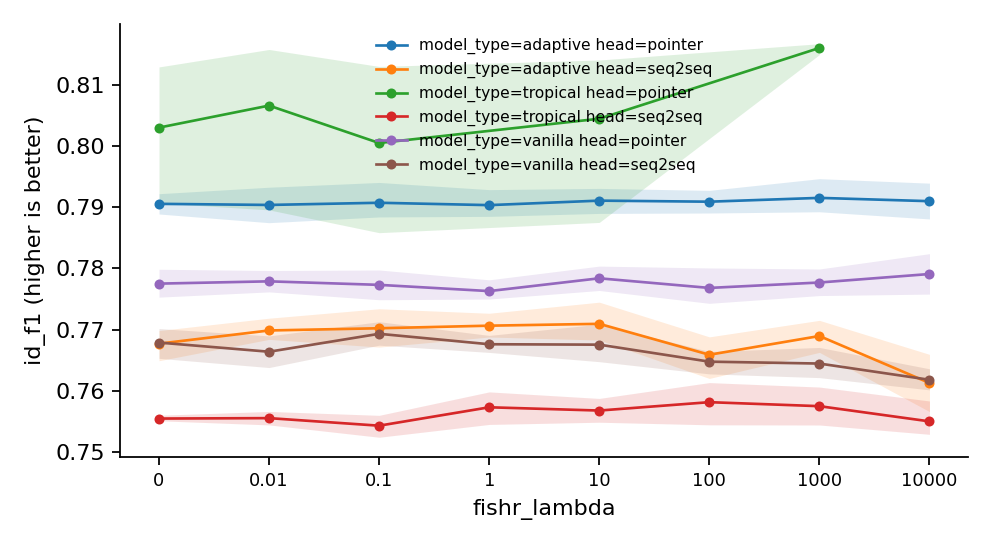
\includegraphics[width=\textwidth]{metric_id_f1.png}
\caption{\texttt{id\_f1} against \texttt{fishr\_lambda}: the mean over seeds with a 95\% bootstrap CI, one line per combination of the other factors.}
\label{fig:id_f1}
\end{figure}

{\small
\begin{longtable}{lllrlrrr}
\caption{\texttt{id\_f1} per cell: mean, 95\% bootstrap CI, SD, seeds, diverged runs.}\label{tab:summary-id_f1}\\
\toprule
\texttt{model\_type} & \texttt{head} & \texttt{fishr\_lambda} & mean & 95\% CI & SD & $n$ & div.\\
\midrule
\endhead
adaptive & pointer & 0 & 0.7906 & [0.789, 0.792] & 0.00221 & 5 & 0\\
adaptive & pointer & 0.01 & 0.7904 & [0.787, 0.793] & 0.00383 & 5 & 0\\
adaptive & pointer & 0.1 & 0.7907 & [0.788, 0.794] & 0.00379 & 5 & 0\\
adaptive & pointer & 1 & 0.7904 & [0.789, 0.793] & 0.00283 & 5 & 0\\
adaptive & pointer & 10 & 0.7911 & [0.789, 0.793] & 0.00252 & 5 & 0\\
adaptive & pointer & 100 & 0.7909 & [0.789, 0.793] & 0.00242 & 5 & 0\\
adaptive & pointer & 1000 & 0.7915 & [0.789, 0.795] & 0.00363 & 5 & 0\\
adaptive & pointer & 1e+04 & 0.791 & [0.788, 0.794] & 0.00398 & 5 & 0\\
adaptive & seq2seq & 0 & 0.7677 & [0.765, 0.77] & 0.00323 & 5 & 0\\
adaptive & seq2seq & 0.01 & 0.7699 & [0.768, 0.772] & 0.00234 & 5 & 0\\
adaptive & seq2seq & 0.1 & 0.7702 & [0.767, 0.773] & 0.00399 & 5 & 0\\
adaptive & seq2seq & 1 & 0.7706 & [0.769, 0.773] & 0.00261 & 5 & 0\\
adaptive & seq2seq & 10 & 0.7709 & [0.768, 0.774] & 0.00403 & 5 & 0\\
adaptive & seq2seq & 100 & 0.7659 & [0.762, 0.769] & 0.00438 & 5 & 0\\
adaptive & seq2seq & 1000 & 0.7689 & [0.766, 0.772] & 0.0036 & 5 & 0\\
adaptive & seq2seq & 1e+04 & 0.7613 & [0.757, 0.766] & 0.00593 & 5 & 0\\
tropical & pointer & 0 & 0.803 & [0.791, 0.813] & 0.0148 & 5 & 0\\
tropical & pointer & 0.01 & 0.8066 & [0.79, 0.816] & 0.017 & 4 & 0\\
tropical & pointer & 0.1 & 0.8005 & [0.786, 0.813] & 0.0171 & 4 & 0\\
tropical & pointer & 10 & 0.8045 & [0.788, 0.814] & 0.0168 & 4 & 0\\
tropical & pointer & 1000 & 0.8161 & [0.815, 0.817] & $9.54\times10^{-4}$ & 3 & 0\\
tropical & seq2seq & 0 & 0.7554 & [0.755, 0.756] & $6.04\times10^{-4}$ & 5 & 0\\
tropical & seq2seq & 0.01 & 0.7555 & [0.754, 0.757] & 0.00147 & 5 & 0\\
tropical & seq2seq & 0.1 & 0.7543 & [0.752, 0.756] & 0.00228 & 5 & 0\\
tropical & seq2seq & 1 & 0.7573 & [0.754, 0.76] & 0.00339 & 5 & 0\\
tropical & seq2seq & 10 & 0.7568 & [0.755, 0.759] & 0.00263 & 5 & 0\\
tropical & seq2seq & 100 & 0.7581 & [0.754, 0.761] & 0.00432 & 5 & 0\\
tropical & seq2seq & 1000 & 0.7575 & [0.754, 0.761] & 0.0041 & 5 & 0\\
tropical & seq2seq & 1e+04 & 0.755 & [0.753, 0.758] & 0.00365 & 5 & 0\\
vanilla & pointer & 0 & 0.7775 & [0.775, 0.78] & 0.00304 & 5 & 0\\
vanilla & pointer & 0.01 & 0.7779 & [0.776, 0.78] & 0.00242 & 5 & 0\\
vanilla & pointer & 0.1 & 0.7773 & [0.775, 0.78] & 0.00329 & 5 & 0\\
vanilla & pointer & 1 & 0.7763 & [0.775, 0.778] & 0.0021 & 5 & 0\\
vanilla & pointer & 10 & 0.7784 & [0.776, 0.78] & 0.00268 & 5 & 0\\
vanilla & pointer & 100 & 0.7768 & [0.774, 0.78] & 0.00371 & 5 & 0\\
vanilla & pointer & 1000 & 0.7777 & [0.776, 0.78] & 0.00291 & 5 & 0\\
vanilla & pointer & 1e+04 & 0.7791 & [0.776, 0.782] & 0.00441 & 5 & 0\\
vanilla & seq2seq & 0 & 0.7679 & [0.765, 0.77] & 0.00313 & 5 & 0\\
vanilla & seq2seq & 0.01 & 0.7664 & [0.764, 0.769] & 0.00336 & 5 & 0\\
vanilla & seq2seq & 0.1 & 0.7693 & [0.767, 0.771] & 0.00255 & 5 & 0\\
vanilla & seq2seq & 1 & 0.7676 & [0.766, 0.769] & 0.00182 & 5 & 0\\
vanilla & seq2seq & 10 & 0.7675 & [0.765, 0.771] & 0.00407 & 5 & 0\\
vanilla & seq2seq & 100 & 0.7647 & [0.763, 0.766] & 0.00234 & 5 & 0\\
vanilla & seq2seq & 1000 & 0.7644 & [0.762, 0.767] & 0.00329 & 5 & 0\\
vanilla & seq2seq & 1e+04 & 0.7618 & [0.76, 0.764] & 0.00233 & 5 & 0\\
\bottomrule
\end{longtable}
}

{\small
\begin{longtable}{lllrrrl}
\caption{\texttt{id\_f1}: each level of \texttt{fishr\_lambda} against its control (0), within each combination of the other factors. parametric: Dunnett vs control.}\label{tab:control-id_f1}\\
\toprule
\texttt{model\_type} & \texttt{head} & \texttt{fishr\_lambda} & difference & 95\% CI & $p$ & \\
\midrule
\endhead
adaptive & pointer & 0.01 & $-1.796\times10^{-4}$ & [-0.00581, 0.00545] & 1.0000 & \\
adaptive & pointer & 0.1 & $1.776\times10^{-4}$ & [-0.00545, 0.00581] & 1.0000 & \\
adaptive & pointer & 1 & $-2.097\times10^{-4}$ & [-0.00584, 0.00542] & 1.0000 & \\
adaptive & pointer & 10 & $5.255\times10^{-4}$ & [-0.00511, 0.00616] & 0.9999 & \\
adaptive & pointer & 100 & $3.523\times10^{-4}$ & [-0.00528, 0.00598] & 1.0000 & \\
adaptive & pointer & 1000 & $9.769\times10^{-4}$ & [-0.00465, 0.00661] & 0.9964 & \\
adaptive & pointer & 1e+04 & $4.365\times10^{-4}$ & [-0.00519, 0.00607] & 1.0000 & \\
adaptive & seq2seq & 0.01 & 0.00216 & [-0.00467, 0.00899] & 0.9159 & \\
adaptive & seq2seq & 0.1 & 0.002521 & [-0.00431, 0.00935] & 0.8435 & \\
adaptive & seq2seq & 1 & 0.002943 & [-0.00389, 0.00977] & 0.7353 & \\
adaptive & seq2seq & 10 & 0.003245 & [-0.00358, 0.0101] & 0.6497 & \\
adaptive & seq2seq & 100 & -0.001813 & [-0.00864, 0.00502] & 0.9626 & \\
adaptive & seq2seq & 1000 & 0.001252 & [-0.00558, 0.00808] & 0.9950 & \\
adaptive & seq2seq & 1e+04 & -0.006432 & [-0.0133, $3.97\times10^{-4}$] & 0.0716 & \\
tropical & pointer & 0.01 & 0.003604 & [-0.0244, 0.0316] & 0.9905 & \\
tropical & pointer & 0.1 & -0.00252 & [-0.0306, 0.0255] & 0.9976 & \\
tropical & pointer & 10 & 0.001453 & [-0.0266, 0.0295] & 0.9997 & \\
tropical & pointer & 1000 & 0.01303 & [-0.0175, 0.0436] & 0.6210 & \\
tropical & seq2seq & 0.01 & $6.986\times10^{-5}$ & [-0.00527, 0.00541] & 1.0000 & \\
tropical & seq2seq & 0.1 & -0.001167 & [-0.00651, 0.00418] & 0.9865 & \\
tropical & seq2seq & 1 & 0.001844 & [-0.0035, 0.00719] & 0.8790 & \\
tropical & seq2seq & 10 & 0.001311 & [-0.00403, 0.00665] & 0.9748 & \\
tropical & seq2seq & 100 & 0.002681 & [-0.00266, 0.00802] & 0.5977 & \\
tropical & seq2seq & 1000 & 0.002027 & [-0.00332, 0.00737] & 0.8269 & \\
tropical & seq2seq & 1e+04 & $-4.617\times10^{-4}$ & [-0.0058, 0.00488] & 1.0000 & \\
vanilla & pointer & 0.01 & $3.744\times10^{-4}$ & [-0.00512, 0.00587] & 1.0000 & \\
vanilla & pointer & 0.1 & $-2.022\times10^{-4}$ & [-0.0057, 0.00529] & 1.0000 & \\
vanilla & pointer & 1 & -0.001222 & [-0.00671, 0.00427] & 0.9851 & \\
vanilla & pointer & 10 & $8.717\times10^{-4}$ & [-0.00462, 0.00636] & 0.9979 & \\
vanilla & pointer & 100 & $-7.031\times10^{-4}$ & [-0.0062, 0.00479] & 0.9995 & \\
vanilla & pointer & 1000 & $1.817\times10^{-4}$ & [-0.00531, 0.00567] & 1.0000 & \\
vanilla & pointer & 1e+04 & 0.001573 & [-0.00392, 0.00707] & 0.9463 & \\
vanilla & seq2seq & 0.01 & -0.001499 & [-0.00664, 0.00364] & 0.9413 & \\
vanilla & seq2seq & 0.1 & 0.001436 & [-0.0037, 0.00657] & 0.9520 & \\
vanilla & seq2seq & 1 & $-2.732\times10^{-4}$ & [-0.00541, 0.00486] & 1.0000 & \\
vanilla & seq2seq & 10 & $-3.401\times10^{-4}$ & [-0.00548, 0.0048] & 1.0000 & \\
vanilla & seq2seq & 100 & -0.003122 & [-0.00826, 0.00201] & 0.4026 & \\
vanilla & seq2seq & 1000 & -0.003432 & [-0.00857, 0.0017] & 0.3096 & \\
vanilla & seq2seq & 1e+04 & -0.006088 & [-0.0112, $-9.51\times10^{-4}$] & 0.0147 & *\\
\bottomrule
\end{longtable}
}

{\small
\begin{longtable}{llrrrrr}
\caption{\texttt{id\_f1} against log10 \texttt{fishr\_lambda}: parametric: OLS slope t-test, seed-bootstrap CI, with the Jonckheere--Terpstra ordered-trend $\tau$ and $p$.}\label{tab:trend-id_f1}\\
\toprule
\texttt{model\_type} & \texttt{head} & estimate & 95\% CI & $p$ & JT $\tau$ & JT $p$\\
\midrule
\endhead
adaptive & pointer & $1.432\times10^{-4}$ & [$5.39\times10^{-5}$, $2.16\times10^{-4}$] & 0.5874 & 0.101 & 0.4577\\
adaptive & seq2seq & -0.001181 & [-0.00157, $-8.40\times10^{-4}$] & 0.0029 & -0.341 & 0.0094\\
tropical & pointer & 0.001984 & [$4.59\times10^{-5}$, 0.00486] & 0.3540 & 0.238 & 0.3293\\
tropical & seq2seq & $2.011\times10^{-4}$ & [$-1.98\times10^{-4}$, $7.55\times10^{-4}$] & 0.4726 & 0.101 & 0.4493\\
vanilla & pointer & $1.743\times10^{-4}$ & [$-4.26\times10^{-6}$, $3.53\times10^{-4}$] & 0.5000 & 0.0476 & 0.7445\\
vanilla & seq2seq & $-9.412\times10^{-4}$ & [-0.00147, $-4.13\times10^{-4}$] & 0.0008 & -0.455 & 0.0010\\
\bottomrule
\end{longtable}
}

{\small
\begin{longtable}{lrrrl}
\caption{\texttt{id\_f1}: paired contrasts by seed, Holm-corrected across the cells. parametric: paired t-test by seed, Holm.}\label{tab:paired-id_f1}\\
\toprule
contrast (within) & difference & 95\% CI & $p$ & \\
\midrule
\endhead
\stackcell{model\_type: tropical - vanilla\\\footnotesize head=pointer fishr\_lambda=0 } & 0.02553 & [0.00515, 0.0459] & 0.1778 & \\
\stackcell{model\_type: tropical - vanilla\\\footnotesize head=pointer fishr\_lambda=0.01 } & 0.02819 & [-0.00199, 0.0584] & 0.2114 & \\
\stackcell{model\_type: tropical - vanilla\\\footnotesize head=pointer fishr\_lambda=0.1 } & 0.02291 & [-0.00765, 0.0535] & 0.2114 & \\
\stackcell{model\_type: tropical - vanilla\\\footnotesize head=pointer fishr\_lambda=10 } & 0.02675 & [-0.00267, 0.0562] & 0.2114 & \\
\stackcell{model\_type: tropical - vanilla\\\footnotesize head=pointer fishr\_lambda=1000 } & 0.04032 & [0.0354, 0.0452] & 0.0096 & *\\
\stackcell{model\_type: tropical - vanilla\\\footnotesize head=seq2seq fishr\_lambda=0 } & -0.01243 & [-0.0162, -0.00863] & 0.0096 & *\\
\stackcell{model\_type: tropical - vanilla\\\footnotesize head=seq2seq fishr\_lambda=0.01 } & -0.01086 & [-0.0154, -0.00628] & 0.0275 & *\\
\stackcell{model\_type: tropical - vanilla\\\footnotesize head=seq2seq fishr\_lambda=0.1 } & -0.01503 & [-0.0189, -0.0112] & 0.0054 & *\\
\stackcell{model\_type: tropical - vanilla\\\footnotesize head=seq2seq fishr\_lambda=1 } & -0.01031 & [-0.0149, -0.0057] & 0.0310 & *\\
\stackcell{model\_type: tropical - vanilla\\\footnotesize head=seq2seq fishr\_lambda=10 } & -0.01078 & [-0.0168, -0.00473] & 0.0621 & \\
\stackcell{model\_type: tropical - vanilla\\\footnotesize head=seq2seq fishr\_lambda=100 } & -0.006629 & [-0.0123, $-9.92\times10^{-4}$] & 0.1855 & \\
\stackcell{model\_type: tropical - vanilla\\\footnotesize head=seq2seq fishr\_lambda=1000 } & -0.006973 & [-0.0141, $1.38\times10^{-4}$] & 0.2114 & \\
\stackcell{model\_type: tropical - vanilla\\\footnotesize head=seq2seq fishr\_lambda=1e+04 } & -0.006806 & [-0.0132, $-4.61\times10^{-4}$] & 0.2041 & \\
\stackcell{model\_type: adaptive - vanilla\\\footnotesize head=pointer fishr\_lambda=0 } & 0.01305 & [0.0101, 0.016] & 0.0034 & *\\
\stackcell{model\_type: adaptive - vanilla\\\footnotesize head=pointer fishr\_lambda=0.01 } & 0.0125 & [0.00903, 0.016] & 0.0062 & *\\
\stackcell{model\_type: adaptive - vanilla\\\footnotesize head=pointer fishr\_lambda=0.1 } & 0.01343 & [0.00855, 0.0183] & 0.0158 & *\\
\stackcell{model\_type: adaptive - vanilla\\\footnotesize head=pointer fishr\_lambda=1 } & 0.01406 & [0.0119, 0.0163] & 0.0009 & *\\
\stackcell{model\_type: adaptive - vanilla\\\footnotesize head=pointer fishr\_lambda=10 } & 0.01271 & [0.00927, 0.0161] & 0.0061 & *\\
\stackcell{model\_type: adaptive - vanilla\\\footnotesize head=pointer fishr\_lambda=100 } & 0.01411 & [0.0104, 0.0178] & 0.0057 & *\\
\stackcell{model\_type: adaptive - vanilla\\\footnotesize head=pointer fishr\_lambda=1000 } & 0.01385 & [0.0118, 0.0159] & 0.0007 & *\\
\stackcell{model\_type: adaptive - vanilla\\\footnotesize head=pointer fishr\_lambda=1e+04 } & 0.01192 & [0.00515, 0.0187] & 0.0722 & \\
\stackcell{model\_type: adaptive - vanilla\\\footnotesize head=seq2seq fishr\_lambda=0 } & $-1.788\times10^{-4}$ & [-0.00704, 0.00668] & 1.0000 & \\
\stackcell{model\_type: adaptive - vanilla\\\footnotesize head=seq2seq fishr\_lambda=0.01 } & 0.00348 & [-0.00278, 0.00974] & 0.9885 & \\
\stackcell{model\_type: adaptive - vanilla\\\footnotesize head=seq2seq fishr\_lambda=0.1 } & $9.065\times10^{-4}$ & [-0.00336, 0.00517] & 1.0000 & \\
\stackcell{model\_type: adaptive - vanilla\\\footnotesize head=seq2seq fishr\_lambda=1 } & 0.003038 & [0.00132, 0.00476] & 0.0722 & \\
\stackcell{model\_type: adaptive - vanilla\\\footnotesize head=seq2seq fishr\_lambda=10 } & 0.003407 & [$6.83\times10^{-4}$, 0.00613] & 0.1787 & \\
\stackcell{model\_type: adaptive - vanilla\\\footnotesize head=seq2seq fishr\_lambda=100 } & 0.001131 & [-0.006, 0.00827] & 1.0000 & \\
\stackcell{model\_type: adaptive - vanilla\\\footnotesize head=seq2seq fishr\_lambda=1000 } & 0.004505 & [$8.22\times10^{-4}$, 0.00819] & 0.1787 & \\
\stackcell{model\_type: adaptive - vanilla\\\footnotesize head=seq2seq fishr\_lambda=1e+04 } & $-5.233\times10^{-4}$ & [-0.00835, 0.00731] & 1.0000 & \\
\stackcell{head: pointer - seq2seq\\\footnotesize model\_type=adaptive fishr\_lambda=0 } & 0.02288 & [0.0168, 0.0289] & 0.0064 & *\\
\stackcell{head: pointer - seq2seq\\\footnotesize model\_type=adaptive fishr\_lambda=0.01 } & 0.02054 & [0.0175, 0.0236] & 0.0009 & *\\
\stackcell{head: pointer - seq2seq\\\footnotesize model\_type=adaptive fishr\_lambda=0.1 } & 0.02053 & [0.0159, 0.0251] & 0.0039 & *\\
\stackcell{head: pointer - seq2seq\\\footnotesize model\_type=adaptive fishr\_lambda=1 } & 0.01972 & [0.0187, 0.0208] & $<10^{-4}$ & *\\
\stackcell{head: pointer - seq2seq\\\footnotesize model\_type=adaptive fishr\_lambda=10 } & 0.02016 & [0.0178, 0.0225] & 0.0003 & *\\
\stackcell{head: pointer - seq2seq\\\footnotesize model\_type=adaptive fishr\_lambda=100 } & 0.02504 & [0.0171, 0.0329] & 0.0120 & *\\
\stackcell{head: pointer - seq2seq\\\footnotesize model\_type=adaptive fishr\_lambda=1000 } & 0.0226 & [0.0194, 0.0258] & 0.0008 & *\\
\stackcell{head: pointer - seq2seq\\\footnotesize model\_type=adaptive fishr\_lambda=1e+04 } & 0.02975 & [0.0223, 0.0372] & 0.0057 & *\\
\stackcell{head: pointer - seq2seq\\\footnotesize model\_type=tropical fishr\_lambda=0 } & 0.0476 & [0.0285, 0.0667] & 0.0229 & *\\
\stackcell{head: pointer - seq2seq\\\footnotesize model\_type=tropical fishr\_lambda=0.01 } & 0.05063 & [0.0242, 0.0771] & 0.0443 & *\\
\stackcell{head: pointer - seq2seq\\\footnotesize model\_type=tropical fishr\_lambda=0.1 } & 0.04548 & [0.0168, 0.0742] & 0.0443 & *\\
\stackcell{head: pointer - seq2seq\\\footnotesize model\_type=tropical fishr\_lambda=10 } & 0.04853 & [0.0207, 0.0763] & 0.0443 & *\\
\stackcell{head: pointer - seq2seq\\\footnotesize model\_type=tropical fishr\_lambda=1000 } & 0.06124 & [0.0525, 0.07] & 0.0132 & *\\
\stackcell{head: pointer - seq2seq\\\footnotesize model\_type=vanilla fishr\_lambda=0 } & 0.009645 & [0.00529, 0.014] & 0.0304 & *\\
\stackcell{head: pointer - seq2seq\\\footnotesize model\_type=vanilla fishr\_lambda=0.01 } & 0.01152 & [0.0054, 0.0176] & 0.0383 & *\\
\stackcell{head: pointer - seq2seq\\\footnotesize model\_type=vanilla fishr\_lambda=0.1 } & 0.008007 & [0.00236, 0.0137] & 0.0443 & *\\
\stackcell{head: pointer - seq2seq\\\footnotesize model\_type=vanilla fishr\_lambda=1 } & 0.008697 & [0.00679, 0.0106] & 0.0038 & *\\
\stackcell{head: pointer - seq2seq\\\footnotesize model\_type=vanilla fishr\_lambda=10 } & 0.01086 & [0.00453, 0.0172] & 0.0443 & *\\
\stackcell{head: pointer - seq2seq\\\footnotesize model\_type=vanilla fishr\_lambda=100 } & 0.01206 & [0.00669, 0.0174] & 0.0304 & *\\
\stackcell{head: pointer - seq2seq\\\footnotesize model\_type=vanilla fishr\_lambda=1000 } & 0.01326 & [0.00701, 0.0195] & 0.0304 & *\\
\stackcell{head: pointer - seq2seq\\\footnotesize model\_type=vanilla fishr\_lambda=1e+04 } & 0.01731 & [0.0109, 0.0237] & 0.0185 & *\\
\bottomrule
\end{longtable}
}

\subsection{\texttt{id\_exact}}
\begin{figure}[tbp]
\centering
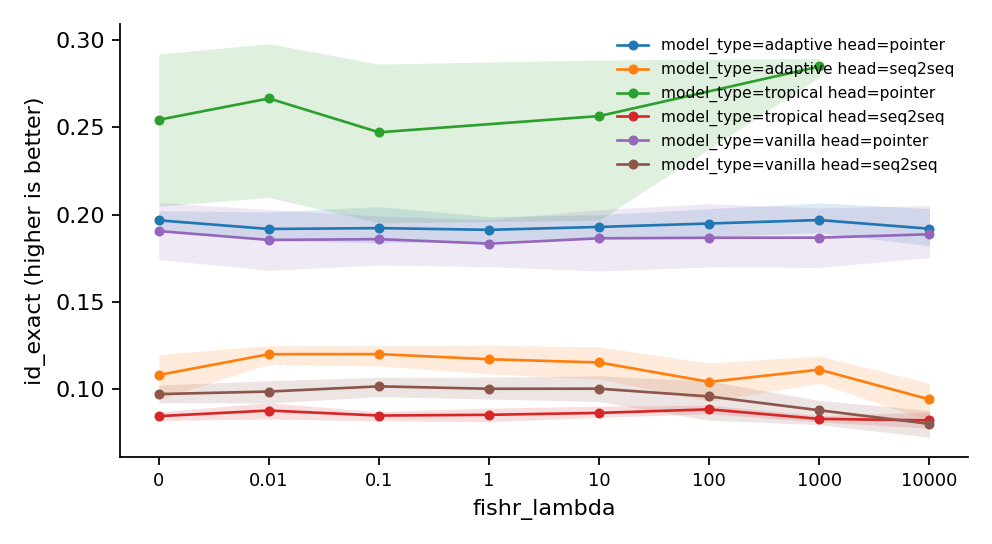
\includegraphics[width=\textwidth]{metric_id_exact.png}
\caption{\texttt{id\_exact} against \texttt{fishr\_lambda}: the mean over seeds with a 95\% bootstrap CI, one line per combination of the other factors.}
\label{fig:id_exact}
\end{figure}

{\small
\begin{longtable}{lllrlrrr}
\caption{\texttt{id\_exact} per cell: mean, 95\% bootstrap CI, SD, seeds, diverged runs.}\label{tab:summary-id_exact}\\
\toprule
\texttt{model\_type} & \texttt{head} & \texttt{fishr\_lambda} & mean & 95\% CI & SD & $n$ & div.\\
\midrule
\endhead
adaptive & pointer & 0 & 0.1967 & [0.192, 0.202] & 0.00674 & 5 & 0\\
adaptive & pointer & 0.01 & 0.1917 & [0.185, 0.202] & 0.011 & 5 & 0\\
adaptive & pointer & 0.1 & 0.1922 & [0.184, 0.205] & 0.0139 & 5 & 0\\
adaptive & pointer & 1 & 0.1912 & [0.185, 0.199] & 0.00922 & 5 & 0\\
adaptive & pointer & 10 & 0.1929 & [0.187, 0.2] & 0.00863 & 5 & 0\\
adaptive & pointer & 100 & 0.1949 & [0.187, 0.203] & 0.01 & 5 & 0\\
adaptive & pointer & 1000 & 0.1969 & [0.19, 0.207] & 0.0113 & 5 & 0\\
adaptive & pointer & 1e+04 & 0.1919 & [0.182, 0.203] & 0.014 & 5 & 0\\
adaptive & seq2seq & 0 & 0.1079 & [0.0938, 0.12] & 0.0171 & 5 & 0\\
adaptive & seq2seq & 0.01 & 0.1198 & [0.114, 0.125] & 0.00729 & 5 & 0\\
adaptive & seq2seq & 0.1 & 0.1199 & [0.113, 0.125] & 0.00826 & 5 & 0\\
adaptive & seq2seq & 1 & 0.117 & [0.109, 0.125] & 0.0116 & 5 & 0\\
adaptive & seq2seq & 10 & 0.1151 & [0.106, 0.124] & 0.012 & 5 & 0\\
adaptive & seq2seq & 100 & 0.1039 & [0.0927, 0.115] & 0.014 & 5 & 0\\
adaptive & seq2seq & 1000 & 0.111 & [0.103, 0.119] & 0.0104 & 5 & 0\\
adaptive & seq2seq & 1e+04 & 0.09386 & [0.0817, 0.103] & 0.014 & 5 & 0\\
tropical & pointer & 0 & 0.2544 & [0.205, 0.292] & 0.0577 & 5 & 0\\
tropical & pointer & 0.01 & 0.2667 & [0.21, 0.298] & 0.0568 & 4 & 0\\
tropical & pointer & 0.1 & 0.2472 & [0.195, 0.286] & 0.0572 & 4 & 0\\
tropical & pointer & 10 & 0.2566 & [0.197, 0.289] & 0.0596 & 4 & 0\\
tropical & pointer & 1000 & 0.285 & [0.279, 0.29] & 0.00551 & 3 & 0\\
tropical & seq2seq & 0 & 0.08428 & [0.0817, 0.0868] & 0.00326 & 5 & 0\\
tropical & seq2seq & 0.01 & 0.0875 & [0.0826, 0.092] & 0.0059 & 5 & 0\\
tropical & seq2seq & 0.1 & 0.08462 & [0.0816, 0.0869] & 0.00335 & 5 & 0\\
tropical & seq2seq & 1 & 0.08504 & [0.0811, 0.0889] & 0.00513 & 5 & 0\\
tropical & seq2seq & 10 & 0.08614 & [0.0836, 0.09] & 0.00447 & 5 & 0\\
tropical & seq2seq & 100 & 0.08818 & [0.0857, 0.0905] & 0.00329 & 5 & 0\\
tropical & seq2seq & 1000 & 0.0827 & [0.0809, 0.0846] & 0.00238 & 5 & 0\\
tropical & seq2seq & 1e+04 & 0.08186 & [0.0774, 0.0866] & 0.0062 & 5 & 0\\
vanilla & pointer & 0 & 0.1905 & [0.174, 0.207] & 0.0214 & 5 & 0\\
vanilla & pointer & 0.01 & 0.1854 & [0.168, 0.203] & 0.0211 & 5 & 0\\
vanilla & pointer & 0.1 & 0.1859 & [0.171, 0.199] & 0.0183 & 5 & 0\\
vanilla & pointer & 1 & 0.1833 & [0.17, 0.197] & 0.0176 & 5 & 0\\
vanilla & pointer & 10 & 0.1864 & [0.168, 0.203] & 0.0223 & 5 & 0\\
vanilla & pointer & 100 & 0.1867 & [0.17, 0.206] & 0.0226 & 5 & 0\\
vanilla & pointer & 1000 & 0.1867 & [0.17, 0.204] & 0.0224 & 5 & 0\\
vanilla & pointer & 1e+04 & 0.1887 & [0.175, 0.205] & 0.0191 & 5 & 0\\
vanilla & seq2seq & 0 & 0.09694 & [0.0921, 0.102] & 0.00644 & 5 & 0\\
vanilla & seq2seq & 0.01 & 0.0984 & [0.0919, 0.105] & 0.00875 & 5 & 0\\
vanilla & seq2seq & 0.1 & 0.1014 & [0.0955, 0.107] & 0.00734 & 5 & 0\\
vanilla & seq2seq & 1 & 0.1 & [0.0941, 0.107] & 0.00793 & 5 & 0\\
vanilla & seq2seq & 10 & 0.1 & [0.0927, 0.107] & 0.00961 & 5 & 0\\
vanilla & seq2seq & 100 & 0.09558 & [0.0819, 0.104] & 0.0147 & 5 & 0\\
vanilla & seq2seq & 1000 & 0.08764 & [0.0794, 0.0933] & 0.00951 & 5 & 0\\
vanilla & seq2seq & 1e+04 & 0.07986 & [0.0722, 0.0876] & 0.0102 & 5 & 0\\
\bottomrule
\end{longtable}
}

{\small
\begin{longtable}{lllrrrl}
\caption{\texttt{id\_exact}: each level of \texttt{fishr\_lambda} against its control (0), within each combination of the other factors. parametric: Dunnett vs control.}\label{tab:control-id_exact}\\
\toprule
\texttt{model\_type} & \texttt{head} & \texttt{fishr\_lambda} & difference & 95\% CI & $p$ & \\
\midrule
\endhead
adaptive & pointer & 0.01 & -0.00498 & [-0.0239, 0.014] & 0.9645 & \\
adaptive & pointer & 0.1 & -0.00448 & [-0.0234, 0.0145] & 0.9794 & \\
adaptive & pointer & 1 & -0.00546 & [-0.0244, 0.0135] & 0.9448 & \\
adaptive & pointer & 10 & -0.0038 & [-0.0228, 0.0152] & 0.9916 & \\
adaptive & pointer & 100 & -0.00184 & [-0.0208, 0.0171] & 0.9999 & \\
adaptive & pointer & 1000 & $1.600\times10^{-4}$ & [-0.0188, 0.0191] & 1.0000 & \\
adaptive & pointer & 1e+04 & -0.00484 & [-0.0238, 0.0141] & 0.9692 & \\
adaptive & seq2seq & 0.01 & 0.01194 & [-0.00938, 0.0333] & 0.4868 & \\
adaptive & seq2seq & 0.1 & 0.01198 & [-0.00934, 0.0333] & 0.4834 & \\
adaptive & seq2seq & 1 & 0.00906 & [-0.0123, 0.0304] & 0.7468 & \\
adaptive & seq2seq & 10 & 0.00718 & [-0.0141, 0.0285] & 0.8906 & \\
adaptive & seq2seq & 100 & -0.00396 & [-0.0253, 0.0174] & 0.9946 & \\
adaptive & seq2seq & 1000 & 0.00306 & [-0.0183, 0.0244] & 0.9989 & \\
adaptive & seq2seq & 1e+04 & -0.01404 & [-0.0354, 0.00728] & 0.3235 & \\
tropical & pointer & 0.01 & 0.01227 & [-0.0871, 0.112] & 0.9918 & \\
tropical & pointer & 0.1 & -0.007175 & [-0.107, 0.0922] & 0.9990 & \\
tropical & pointer & 10 & 0.00215 & [-0.0972, 0.102] & 1.0000 & \\
tropical & pointer & 1000 & 0.0306 & [-0.0776, 0.139] & 0.8639 & \\
tropical & seq2seq & 0.01 & 0.00322 & [-0.00454, 0.011] & 0.7649 & \\
tropical & seq2seq & 0.1 & $3.400\times10^{-4}$ & [-0.00742, 0.0081] & 1.0000 & \\
tropical & seq2seq & 1 & $7.600\times10^{-4}$ & [-0.007, 0.00852] & 0.9999 & \\
tropical & seq2seq & 10 & 0.00186 & [-0.0059, 0.00962] & 0.9777 & \\
tropical & seq2seq & 100 & 0.0039 & [-0.00386, 0.0117] & 0.5959 & \\
tropical & seq2seq & 1000 & -0.00158 & [-0.00934, 0.00618] & 0.9908 & \\
tropical & seq2seq & 1e+04 & -0.00242 & [-0.0102, 0.00534] & 0.9208 & \\
vanilla & pointer & 0.01 & -0.0051 & [-0.0412, 0.031] & 0.9990 & \\
vanilla & pointer & 0.1 & -0.00466 & [-0.0408, 0.0315] & 0.9994 & \\
vanilla & pointer & 1 & -0.0072 & [-0.0433, 0.0289] & 0.9919 & \\
vanilla & pointer & 10 & -0.00418 & [-0.0403, 0.0319] & 0.9997 & \\
vanilla & pointer & 100 & -0.00386 & [-0.04, 0.0323] & 0.9998 & \\
vanilla & pointer & 1000 & -0.0038 & [-0.0399, 0.0323] & 0.9998 & \\
vanilla & pointer & 1e+04 & -0.00184 & [-0.038, 0.0343] & 1.0000 & \\
vanilla & seq2seq & 0.01 & 0.00146 & [-0.0153, 0.0182] & 1.0000 & \\
vanilla & seq2seq & 0.1 & 0.00444 & [-0.0123, 0.0212] & 0.9631 & \\
vanilla & seq2seq & 1 & 0.00306 & [-0.0137, 0.0198] & 0.9951 & \\
vanilla & seq2seq & 10 & 0.0031 & [-0.0137, 0.0199] & 0.9948 & \\
vanilla & seq2seq & 100 & -0.00136 & [-0.0181, 0.0154] & 1.0000 & \\
vanilla & seq2seq & 1000 & -0.0093 & [-0.0261, 0.00747] & 0.4969 & \\
vanilla & seq2seq & 1e+04 & -0.01708 & [-0.0339, $-3.08\times10^{-4}$] & 0.0446 & *\\
\bottomrule
\end{longtable}
}

{\small
\begin{longtable}{llrrrrr}
\caption{\texttt{id\_exact} against log10 \texttt{fishr\_lambda}: parametric: OLS slope t-test, seed-bootstrap CI, with the Jonckheere--Terpstra ordered-trend $\tau$ and $p$.}\label{tab:trend-id_exact}\\
\toprule
\texttt{model\_type} & \texttt{head} & estimate & 95\% CI & $p$ & JT $\tau$ & JT $p$\\
\midrule
\endhead
adaptive & pointer & $4.757\times10^{-4}$ & [$3.04\times10^{-4}$, $6.88\times10^{-4}$] & 0.5977 & 0.135 & 0.3053\\
adaptive & seq2seq & -0.003886 & [-0.00518, -0.00294] & 0.0003 & -0.446 & 0.0004\\
tropical & pointer & 0.004053 & [-0.0018, 0.0142] & 0.5702 & -0.167 & 0.5013\\
tropical & seq2seq & $-6.293\times10^{-4}$ & [-0.00153, $2.61\times10^{-4}$] & 0.1148 & -0.217 & 0.1052\\
vanilla & pointer & $5.300\times10^{-4}$ & [$-7.33\times10^{-4}$, 0.00186] & 0.7431 & 0.0457 & 0.7690\\
vanilla & seq2seq & -0.003126 & [-0.00569, $-9.45\times10^{-4}$] & 0.0008 & -0.429 & 0.0004\\
\bottomrule
\end{longtable}
}

{\small
\begin{longtable}{lrrrl}
\caption{\texttt{id\_exact}: paired contrasts by seed, Holm-corrected across the cells. parametric: paired t-test by seed, Holm.}\label{tab:paired-id_exact}\\
\toprule
contrast (within) & difference & 95\% CI & $p$ & \\
\midrule
\endhead
\stackcell{model\_type: tropical - vanilla\\\footnotesize head=pointer fishr\_lambda=0 } & 0.06386 & [-0.0326, 0.16] & 0.8861 & \\
\stackcell{model\_type: tropical - vanilla\\\footnotesize head=pointer fishr\_lambda=0.01 } & 0.0812 & [-0.0419, 0.204] & 0.8861 & \\
\stackcell{model\_type: tropical - vanilla\\\footnotesize head=pointer fishr\_lambda=0.1 } & 0.05835 & [-0.0574, 0.174] & 0.8861 & \\
\stackcell{model\_type: tropical - vanilla\\\footnotesize head=pointer fishr\_lambda=10 } & 0.07135 & [-0.0556, 0.198] & 0.8861 & \\
\stackcell{model\_type: tropical - vanilla\\\footnotesize head=pointer fishr\_lambda=1000 } & 0.1122 & [0.0884, 0.136] & 0.0315 & *\\
\stackcell{model\_type: tropical - vanilla\\\footnotesize head=seq2seq fishr\_lambda=0 } & -0.01266 & [-0.0228, -0.00253] & 0.2559 & \\
\stackcell{model\_type: tropical - vanilla\\\footnotesize head=seq2seq fishr\_lambda=0.01 } & -0.0109 & [-0.0249, 0.00314] & 0.7784 & \\
\stackcell{model\_type: tropical - vanilla\\\footnotesize head=seq2seq fishr\_lambda=0.1 } & -0.01676 & [-0.0289, -0.00459] & 0.2061 & \\
\stackcell{model\_type: tropical - vanilla\\\footnotesize head=seq2seq fishr\_lambda=1 } & -0.01496 & [-0.0251, -0.00478] & 0.1813 & \\
\stackcell{model\_type: tropical - vanilla\\\footnotesize head=seq2seq fishr\_lambda=10 } & -0.0139 & [-0.0293, 0.00149] & 0.5965 & \\
\stackcell{model\_type: tropical - vanilla\\\footnotesize head=seq2seq fishr\_lambda=100 } & -0.0074 & [-0.0264, 0.0116] & 1.0000 & \\
\stackcell{model\_type: tropical - vanilla\\\footnotesize head=seq2seq fishr\_lambda=1000 } & -0.00494 & [-0.0188, 0.00889] & 1.0000 & \\
\stackcell{model\_type: tropical - vanilla\\\footnotesize head=seq2seq fishr\_lambda=1e+04 } & 0.002 & [-0.0177, 0.0217] & 1.0000 & \\
\stackcell{model\_type: adaptive - vanilla\\\footnotesize head=pointer fishr\_lambda=0 } & 0.00616 & [-0.0211, 0.0335] & 1.0000 & \\
\stackcell{model\_type: adaptive - vanilla\\\footnotesize head=pointer fishr\_lambda=0.01 } & 0.00628 & [-0.012, 0.0246] & 1.0000 & \\
\stackcell{model\_type: adaptive - vanilla\\\footnotesize head=pointer fishr\_lambda=0.1 } & 0.00634 & [-0.0104, 0.0231] & 1.0000 & \\
\stackcell{model\_type: adaptive - vanilla\\\footnotesize head=pointer fishr\_lambda=1 } & 0.0079 & [-0.0115, 0.0273] & 1.0000 & \\
\stackcell{model\_type: adaptive - vanilla\\\footnotesize head=pointer fishr\_lambda=10 } & 0.00654 & [-0.0179, 0.0309] & 1.0000 & \\
\stackcell{model\_type: adaptive - vanilla\\\footnotesize head=pointer fishr\_lambda=100 } & 0.00818 & [-0.0156, 0.0319] & 1.0000 & \\
\stackcell{model\_type: adaptive - vanilla\\\footnotesize head=pointer fishr\_lambda=1000 } & 0.01012 & [-0.00689, 0.0271] & 1.0000 & \\
\stackcell{model\_type: adaptive - vanilla\\\footnotesize head=pointer fishr\_lambda=1e+04 } & 0.00316 & [-0.0275, 0.0338] & 1.0000 & \\
\stackcell{model\_type: adaptive - vanilla\\\footnotesize head=seq2seq fishr\_lambda=0 } & 0.01096 & [-0.0136, 0.0355] & 1.0000 & \\
\stackcell{model\_type: adaptive - vanilla\\\footnotesize head=seq2seq fishr\_lambda=0.01 } & 0.02144 & [0.00331, 0.0396] & 0.4258 & \\
\stackcell{model\_type: adaptive - vanilla\\\footnotesize head=seq2seq fishr\_lambda=0.1 } & 0.0185 & [0.00258, 0.0344] & 0.4258 & \\
\stackcell{model\_type: adaptive - vanilla\\\footnotesize head=seq2seq fishr\_lambda=1 } & 0.01696 & [0.00522, 0.0287] & 0.2395 & \\
\stackcell{model\_type: adaptive - vanilla\\\footnotesize head=seq2seq fishr\_lambda=10 } & 0.01504 & [-0.00355, 0.0336] & 1.0000 & \\
\stackcell{model\_type: adaptive - vanilla\\\footnotesize head=seq2seq fishr\_lambda=100 } & 0.00836 & [-0.0191, 0.0358] & 1.0000 & \\
\stackcell{model\_type: adaptive - vanilla\\\footnotesize head=seq2seq fishr\_lambda=1000 } & 0.02332 & [0.0137, 0.033] & 0.0408 & *\\
\stackcell{model\_type: adaptive - vanilla\\\footnotesize head=seq2seq fishr\_lambda=1e+04 } & 0.014 & [-0.00707, 0.0351] & 1.0000 & \\
\stackcell{head: pointer - seq2seq\\\footnotesize model\_type=adaptive fishr\_lambda=0 } & 0.0888 & [0.0684, 0.109] & 0.0043 & *\\
\stackcell{head: pointer - seq2seq\\\footnotesize model\_type=adaptive fishr\_lambda=0.01 } & 0.07188 & [0.0546, 0.0891] & 0.0048 & *\\
\stackcell{head: pointer - seq2seq\\\footnotesize model\_type=adaptive fishr\_lambda=0.1 } & 0.07234 & [0.0541, 0.0906] & 0.0050 & *\\
\stackcell{head: pointer - seq2seq\\\footnotesize model\_type=adaptive fishr\_lambda=1 } & 0.07428 & [0.0583, 0.0903] & 0.0038 & *\\
\stackcell{head: pointer - seq2seq\\\footnotesize model\_type=adaptive fishr\_lambda=10 } & 0.07782 & [0.0701, 0.0855] & 0.0002 & *\\
\stackcell{head: pointer - seq2seq\\\footnotesize model\_type=adaptive fishr\_lambda=100 } & 0.09092 & [0.0617, 0.12] & 0.0065 & *\\
\stackcell{head: pointer - seq2seq\\\footnotesize model\_type=adaptive fishr\_lambda=1000 } & 0.0859 & [0.0737, 0.0981] & 0.0008 & *\\
\stackcell{head: pointer - seq2seq\\\footnotesize model\_type=adaptive fishr\_lambda=1e+04 } & 0.098 & [0.0743, 0.122] & 0.0048 & *\\
\stackcell{head: pointer - seq2seq\\\footnotesize model\_type=tropical fishr\_lambda=0 } & 0.1701 & [0.102, 0.239] & 0.0092 & *\\
\stackcell{head: pointer - seq2seq\\\footnotesize model\_type=tropical fishr\_lambda=0.01 } & 0.1809 & [0.0967, 0.265] & 0.0192 & *\\
\stackcell{head: pointer - seq2seq\\\footnotesize model\_type=tropical fishr\_lambda=0.1 } & 0.1634 & [0.0773, 0.249] & 0.0192 & *\\
\stackcell{head: pointer - seq2seq\\\footnotesize model\_type=tropical fishr\_lambda=10 } & 0.1695 & [0.0755, 0.264] & 0.0192 & *\\
\stackcell{head: pointer - seq2seq\\\footnotesize model\_type=tropical fishr\_lambda=1000 } & 0.2022 & [0.192, 0.212] & 0.0024 & *\\
\stackcell{head: pointer - seq2seq\\\footnotesize model\_type=vanilla fishr\_lambda=0 } & 0.0936 & [0.0674, 0.12] & 0.0052 & *\\
\stackcell{head: pointer - seq2seq\\\footnotesize model\_type=vanilla fishr\_lambda=0.01 } & 0.08704 & [0.0621, 0.112] & 0.0052 & *\\
\stackcell{head: pointer - seq2seq\\\footnotesize model\_type=vanilla fishr\_lambda=0.1 } & 0.0845 & [0.0654, 0.104] & 0.0043 & *\\
\stackcell{head: pointer - seq2seq\\\footnotesize model\_type=vanilla fishr\_lambda=1 } & 0.08334 & [0.0618, 0.105] & 0.0050 & *\\
\stackcell{head: pointer - seq2seq\\\footnotesize model\_type=vanilla fishr\_lambda=10 } & 0.08632 & [0.0642, 0.108] & 0.0050 & *\\
\stackcell{head: pointer - seq2seq\\\footnotesize model\_type=vanilla fishr\_lambda=100 } & 0.0911 & [0.0613, 0.121] & 0.0065 & *\\
\stackcell{head: pointer - seq2seq\\\footnotesize model\_type=vanilla fishr\_lambda=1000 } & 0.0991 & [0.0678, 0.13] & 0.0065 & *\\
\stackcell{head: pointer - seq2seq\\\footnotesize model\_type=vanilla fishr\_lambda=1e+04 } & 0.1088 & [0.0808, 0.137] & 0.0050 & *\\
\bottomrule
\end{longtable}
}


\section{Curves}
\begin{figure}[tbp]
\centering
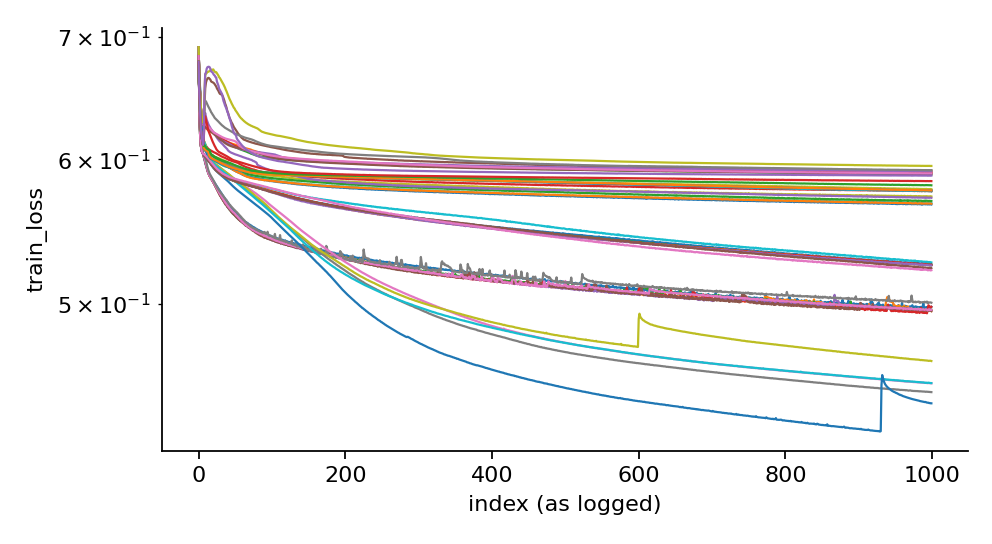
\includegraphics[width=\textwidth]{curve_train_loss.png}
\caption{\texttt{train\_loss}, the mean over seeds per cell.}
\label{fig:curve-1}
\end{figure}
\begin{figure}[tbp]
\centering
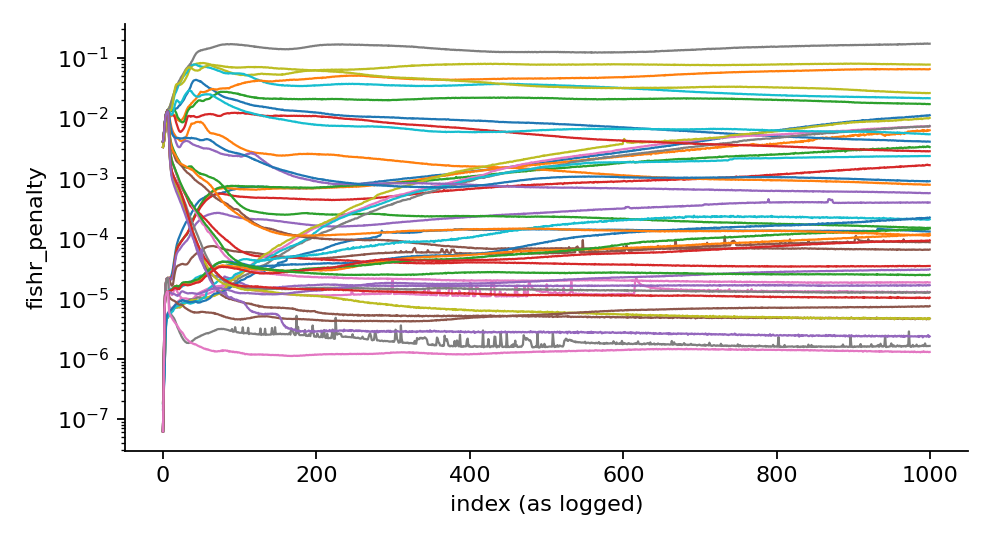
\includegraphics[width=\textwidth]{curve_fishr_penalty.png}
\caption{\texttt{fishr\_penalty}, the mean over seeds per cell.}
\label{fig:curve-2}
\end{figure}
\begin{figure}[tbp]
\centering
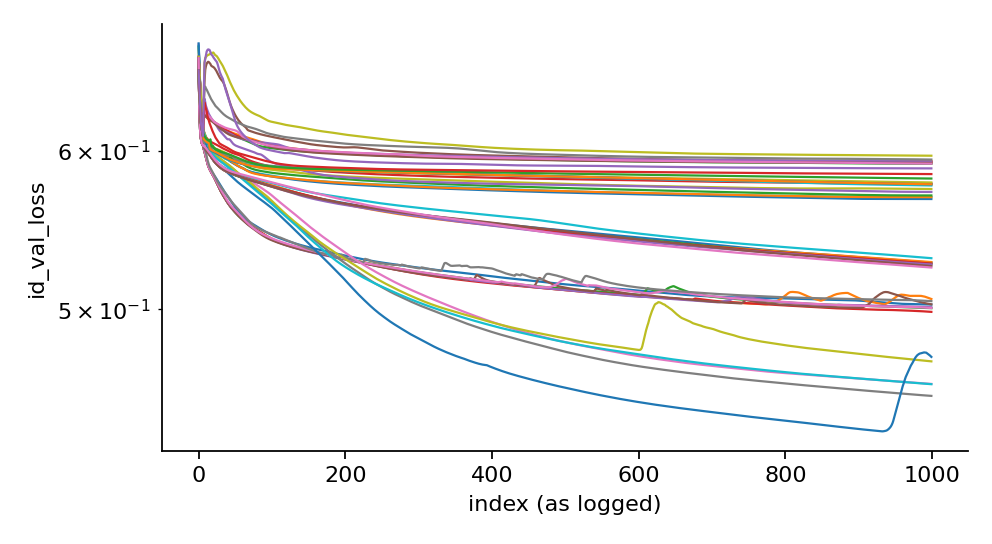
\includegraphics[width=\textwidth]{curve_id_val_loss.png}
\caption{\texttt{id\_val\_loss}, the mean over seeds per cell.}
\label{fig:curve-3}
\end{figure}

\section{Configuration}
The base configuration every run shares (frozen hash \texttt{beab4c1c6902}); factor levels are in \autoref{tab:summary-ood_len_f1}.
{\footnotesize
\begin{verbatim}
task:
  name: BalancedPartitionDataset
  value_range:
  - 1
  - 10
  target_range: null
  weight_range: null
  adversarial_range:
  - 10
  - 30
  noise_prob: 0.0
data:
  train_lengths:
  - 4
  - 5
  - 6
  - 7
  - 8
  ood_lengths:
  - 12
  - 16
  - 64
  ood_value_range:
  - 11
  - 100
  ood_noise_range:
  - 10
  - 30
  ood_noise_prob: 0.5
  n_per_length: 20000
  n_eval_per_length: 2000
  curve_eval_limit: 256
model:
  d_model: 64
  n_heads: 2
  num_layers: 1
  dropout: 0.0
  tropical_impl: legacy
optim:
  lr: 0.0001
  epochs: 1000
  batch_size: 100
  eval_batch_size: 256
fishr:
  ema: 0.95
  anneal_iters: 1500
  reset_optimizer: true
\end{verbatim}
}
Store: \texttt{campaigns/tropical/BalancedPartition/results}.
\end{document}